%!TEX root = skripsi.tex
%-----------------------------------------------------------------------------%
\chapter{\babLima}
%-----------------------------------------------------------------------------%

This chapter focuses on the experiments that we have conducted. Firstly, the data statistics about the semantic role distribution are presented. The experiment scenarios are then explained, followed by the results and analyses of this work.
%-----------------------------------------------------------------------------%

\section{Data Statistics}
As explained in Chapter 3, there are 8 labels to be predicted, which are: \agent, \predicate, \patient, \modal, \beneficiary, \location, \greet, and \timesrl. The distribution of the labels in our data set is presented in Figure~\ref{fig:srldistribution}.

\begin{figure}
	\centering
	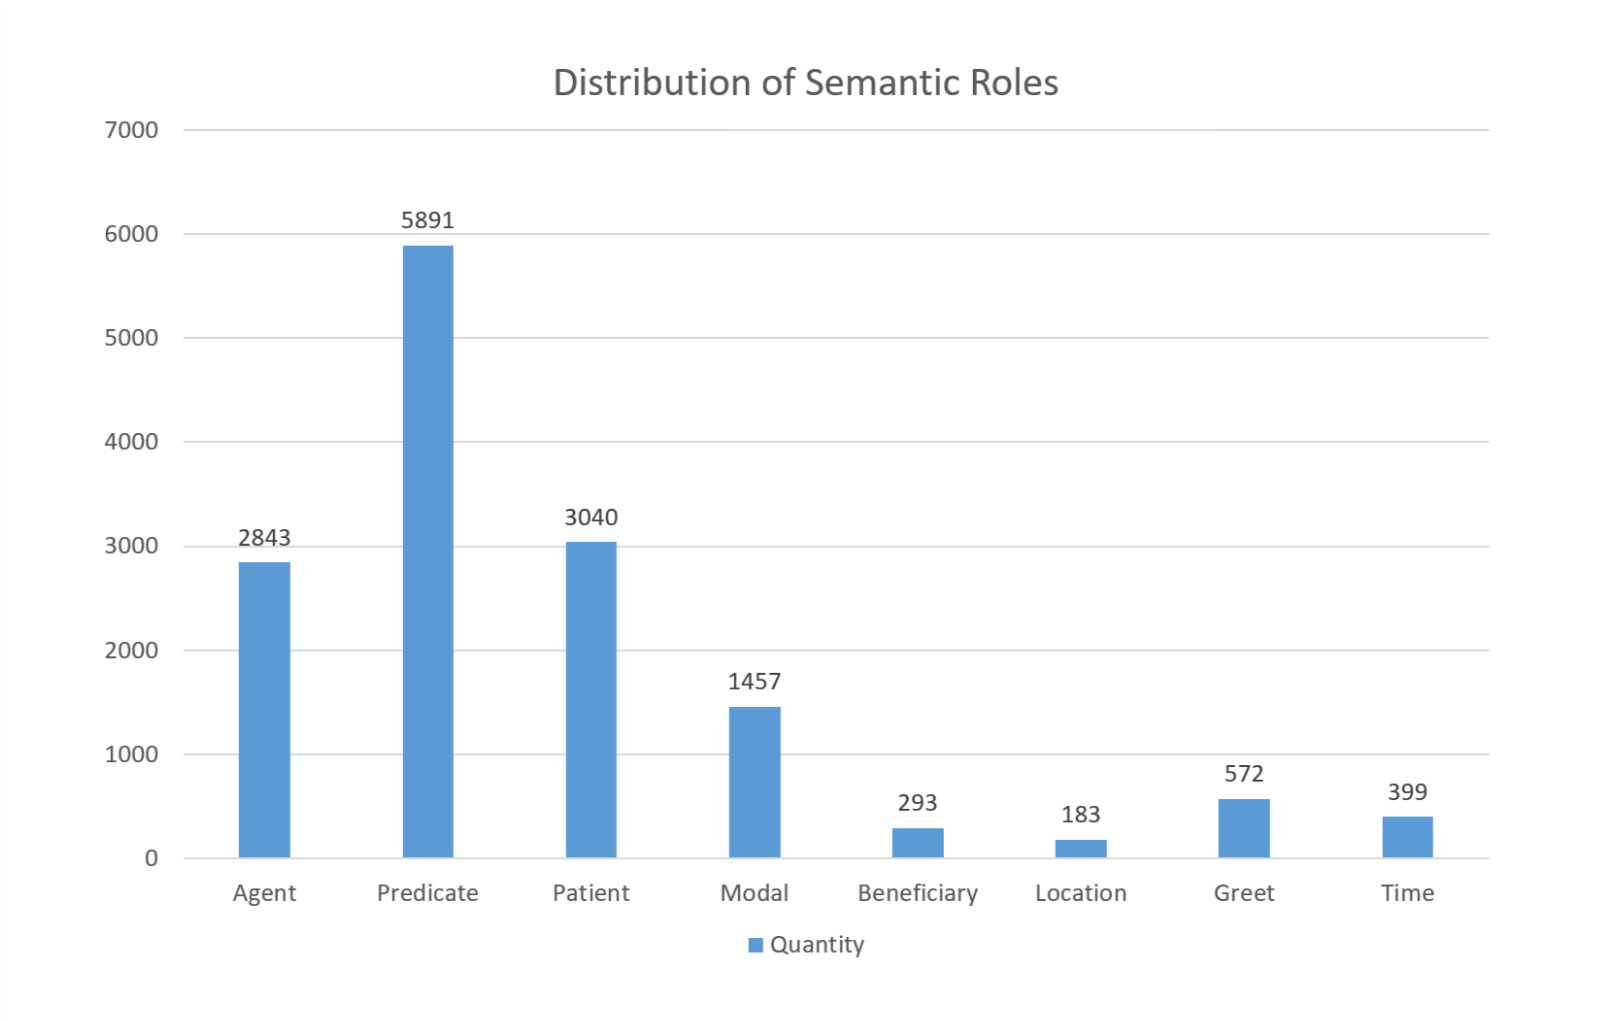
\includegraphics[width=\linewidth]{images/srldistribution}
	\caption{Label Distribution}
	\label{fig:srldistribution}
\end{figure}

\section{Experiment Scenario}
Our experiment consists of two scenario sets: feature selection and model selection. In feature selection, we experiment to find which feature combination outputs the best result. For model selection, the experiment focuses on finding the best model architecture to get the highest result.

The feature selection set consists of 4 combination scenarios, which are:
\begin{enumerate}
	\item Word Embedding (WE)
	\item Word Embedding + Neighboring Word Embeddings (WE + NW)
	\item Word Embedding + POS Tag (WE + POS)
	\item Word Embedding + POS Tag + Neighboring Word Embeddings (WE + POS + NW)
\end{enumerate}

In this scenario set, we use vanilla LSTM for the base architecture. Out of 4 combinations, we pick the best two to be experimented in the model selection scenario set.

The model selection consists of 4 scenario sets. The first set aims to find which feature combination is better when the LSTM layers are added. The next set compares the performance between DBLSTM, DBLSTM-Zhou, and DBLSTM Highway. The third set aims to see the effect of using CNN layer. Lasltly, the fourth set aims to see the impact of our proposed attention layer towards the performance.

\subsection{Scenario 1: Feature Selection}
Table~\ref{tab:feature_scenario} shows the results of the afore-mentioned four feature combinations. The highest result is achieved with the combination of WE + POS + NW, followed by WE + POS, WE + NW, and WE, with F1 scores of 79.76\%, 79.10\%, 73.76\%, and 73.12\%, respectively. 

\begin{table}
	\centering
	\caption{Results (in \%) of Feature Selection Scenario}
	\label{tab:feature_scenario}
	\begin{tabular}{lccc}
		\hline
		Feature & Precision & Recall & F1 \\
		\hline\hline
		WE & 75.20 & 71.16 & 73.12 \\
		WE + NW & 76.07 & 71.58 & 73.76 \\
		WE + POS & \textbf{80.09} & \textbf{78.14} & \textbf{79.10} \\
		WE + POS + NW & \textbf{80.96} & \textbf{78.60} & \textbf{79.76} \\
		\hline
	\end{tabular}

\end{table}

Our first experiment uses only word embedding (WE) as the feature. For a starting point, the results are promising with 75.20\% precision, 71.16\% recall and 73.12\% F1. Table~\ref{tab:ex11srl} shows the precision, recall, and F1 scores for each semantic role when only word embedding is used as the feature.

% Table ex11srl, ubah ini jadi tabel
\begin{table}
	\centering
	\caption{Precision, Recall, F1 scores (in \%) of each label for scenario WE}
	\label{tab:ex11srl}
	\begin{tabular}{lccc}
		\hline
		Label & Precision & Recall & F1 \\
		\hline\hline
		\agent & 74.53 & 86.74 & 80.17 \\
		\predicate & 88.01 & 89.46 & 88.73 \\
		\patient & 74.30 & 68.68 & 71.38 \\
		\modal & 78.14 & 76.74 & 77.43 \\
		\beneficiary & 68.68 & 66.29 & 67.47 \\
		\location & 68.31 & 55.69 & 61.36 \\
		\greet & 69.13 & 52.08 & 59.40 \\
		\timesrl & 80.58 & 73.61 & 76.94 \\
		\hline
		Average & 75.20 & 71.16 & 73.12\\
		\hline
	\end{tabular}

\end{table}


As we can see from the table above, the top three semantic roles with the highest F1 scores are \predicate~(88.73\%), \agent~(80.17\%), and \modal~(77.43\%). On the other hand, the top three semantic roles with the lowest F1 scores are \greet~(59.40\%), \location~(61.36\%), and \beneficiary~(67.47\%). We suggest that these results are partially caused by the unbalanced distribution of semantic roles as presented in Figure~\ref{fig:srldistribution}. \predicate, \agent, and \modal~ are on the top of the distribution while \greet, \location, and \beneficiary~are among the lowest. When we analyze the prediction results, an interesting finding is found. The model often mispredicts \greet~as \agent~as presented in Table~\ref{tab:contohgreetagent}

\begin{table}
	\centering
	\caption{Misprediction example of \greet~when using only WE as the feature}
	\label{tab:contohgreetagent}
	\begin{tabular}{|l|ccccc|}
		\hline
		\textbf{Sentence} 				& jemma & kamu & kenal & dito & enggak \\
		\hline
		\textbf{Expected}				& \textbf{B-\greet} & B-\agent & B-\predicate & B-\patient  & O\\
		\hline
		\textbf{Predicted}		& \textbf{B-\agent} & B-\agent & B-\predicate & B-\patient  & O\\
		\hline
	\end{tabular}
\end{table}

In this example, "jemma" should be labeled as \greet~while "kamu" should be labeled as \agent. This example illustrates a tricky situation in which the model has to decide which one is the \agent~or \greet~since both are located side by side. The model from our first experiment (WE) cannot differentiate this and therefore, it predicts both "jemma" and "kamu" as \agent. We thus propose to use Neighboring Word Embeddings (NW) as the additional feature. With this new feature, the machine will have the additional information from the surrounding words. In the previous example, the machine can determine that "jemma" should be labeled as \greet~when it knows that the following word is "kamu", which most likely will be an \agent~or \patient in a sentence.

When we try to use Neighboring Word Embeddings (NW) as the additional feature (experiment WE + NW), the F1 result slightly increases from 73.12\% to 73.76\%. The most notable improvement is the label \greet~whose F1 score increases from 59.40\% to 71.41\%. While in the previous experiment (WE), the model mispredicts \greet~as \agent, the model from this experiment (WE + NW) predicts it correctly, as presented in Table~\ref{tab:contohgreetagenttrue}:

\begin{table}
	\centering
	\caption{Correct prediction example of \greet when using WE + NW as the features}
	\label{tab:contohgreetagenttrue}
	\begin{tabular}{|l|ccccc|}
		\hline
		\textbf{Sentence} 				& jemma & kamu & kenal & dito & enggak \\
		\hline
		\textbf{Expected}				& \textbf{B-\greet} & B-\agent & B-\predicate & B-\patient  & O\\
		\hline
		\textbf{Predicted}		& \textbf{B-\greet} & B-\agent & B-\predicate & B-\patient  & O\\
		\hline
	\end{tabular}
\end{table}

This proves that the surrounding words can be a helpful information to distinguish when to predict a token as \greet~or ~\agent.

Another interesting finding that we found in the results of WE experiment is presented in Table~\ref{tab:contohwaktufalse}.

\begin{table}
	\centering
	\caption{Misprediction example of \timesrl~when using WE as the feature}
	\label{tab:contohwaktufalse}
	\begin{tabular}{|l|ccc|}
		\hline
		\textbf{Sentence} 				& skrg & lgi & main \\
		\hline
		\textbf{Expected}				& \textbf{B-\timesrl} & B-\modal & B-\predicate\\
		\hline
		\textbf{Predicted}		& \textbf{O} & B-\modal & B-\predicate \\
		\hline
	\end{tabular}
\end{table}

The example illustrates that the machine does not predict "skrg" (formal: "sekarang") as \timesrl, but rather labels it as "other". This case also happens to other semantic roles including \agent, \patient, \beneficiary, \location, and \greet, where the machine mispredicts them as "other". This may be caused by the wide variety of abbreviations in informal language that the training data may not contain. This is due to the fact that our data set is relatively small (5,035 instances) compared to other SRL data set for formal language, such as ConLL 2005 data set with 39,832 instances~\citep{carreras2005introduction}. For instance, "sekarang" has a lot of informal forms such as "skrg", "skg", and "skrng". Our training data may not contain one of its informal forms, "skrg", and thus, the model mispredicts it as "other". 

To address this issue, we argue that POS tags provide meaningful information to increase all semantic role results. \agent, \patient, \beneficiary, \location, \greet, and \timesrl~are all \textit{nouns}. Adding the POS tag \textit{noun} information will give a hint to the model in order to determine which tokens are the candidates of these semantic roles. In the previous example, the machine may predict "skrg" as \timesrl~if it knows that the word's POS tag is \textit{noun}. In addition, \predicate~is often in a form of \textit{verb}, though in some cases of Indonesian language, the \predicate~is an \textit{adjective}. Therefore, knowing that a token is a verb will help the machine to predict it as a \predicate. Lastly, \modal~is mostly in a form of adverb ("akan", "lagi", "harus"). Adding information that tells a word is an adverb will help the model to predict \modal~as well. Based on this rationale, we believe that POS tag will increase the performance of all semantic roles.

When we add POS tag as our additional feature (experiment WE + POS), the average F1 score increases from 73.12\% (WE) to 79.10\% (WE + POS) as presented in Table~\ref{tab:feature_scenario}. The improvements of all semantic roles when we compare experiment WE and WE + POS are presented in Table~\ref{tab:wevswepos}.

\begin{table}
	\centering
	\caption{Precision, Recall, F1 scores (in \%) of each label for scenario WE and WE + POS}
	\label{tab:wevswepos}
	\begin{tabular}{|l|ccc|ccc|}
		\hline
		& \multicolumn{3}{c}{ WE } & \multicolumn{3}{c}{ WE + POS } \\
		\hline
		Label & Precision & Recall & F1 & Precision & Recall & F1 \\
		\hline\hline
		\agent & 74.53 & 86.74 & 80.17 & 75.03 & 88.93 & 81.39 \\
		\predicate & 88.01 & 89.46 & 88.73 & 96.36 & 97.07 & 96.71 \\
		\patient & 74.30 & 68.68 & 71.38 & 78.48 & 75.57 & 77.00 \\
		\modal & 78.14 & 76.74 & 77.43 & 84.49 & 82.08 & 83.27 \\
		\beneficiary & 68.68 & 66.29 & 67.47 & 73.91 & 71.01 & 72.43 \\
		\location & 68.31 & 55.69 & 61.36 & 72.35 & 67.68 & 69.93 \\
		\greet & 69.13 & 52.08 & 59.40 & 71.28 & 56.01 & 62.73 \\
		\timesrl & 80.58 & 73.61 & 76.94 & 88.87 & 86.78 & 87.81 \\
		\hline
		Average & 75.21 & 71.16 & 73.12 & 80.10 & 78.14 & 79.10 \\
		\hline
	\end{tabular}

\end{table}

All the semantic roles with POS tag \textit{noun} (\agent, \patient, \beneficiary, \location, \greet, and \timesrl) are all having improvements in terms of the F1 scores. The most notable improvements are \timesrl~(76.85\% to 87.72\%), \location~(61.26\% to 69.79\%), and \beneficiary~(66.85\% to 72.02\%). Referring to the previous example, the new model correctly predicts "skrg" as \timesrl rather than "other", as presented in Table~\ref{tab:timetrue}. On the other hand, the \predicate~improves from 88.72\% to 96.71\% while \modal~increases from 77.41\% to 83.21\%. These results prove that POS tag provides a contribution to increase the performance. While most of the deep learning research aims not to use hand-crafted features like POS tag, that is not the case in our work. Our experiment shows that such features are still important when the data set is relatively small. Nonetheless, building a huge data set is also costly, we therefore have to find a workaround in order to achieve competitive results by only using small data set. In this case, the workaround is to add traditional features such as POS tag.

\begin{table}
	\centering
	\caption{Correct prediction example of \timesrl~when using WE + POS as the features}
	\label{tab:timetrue}
	\begin{tabular}{|l|ccc|}
		\hline
		\textbf{Sentence} 				& skrg & lgi & main \\
		\hline
		\textbf{Expected}				& \textbf{B-\timesrl} & B-\modal & B-\predicate\\
		\hline
		\textbf{Predicted}		& \textbf{B-\timesrl} & B-\modal & B-\predicate \\
		\hline
	\end{tabular}
\end{table}

Finally, we try to add Neighboring Words in addition to experiment WE + POS. Hence, the feature combination is WE + POS + NW. The F1 score slightly increases from 79.10\% (WE + POS) to 79.76\% (WE + POS + N). In this improvement, the F1 score of \greet increases from 62.65\% (WE + POS) to 75.02\% (WE + POS + NW). This is the same case as the improvement that we have seen in experiment WE and WE + NW. 

%Surprisingly, when we combine the neighboring words of the argument as in WE + WE-N, the result slightly decreases by 0.08\%, compared to only using WE feature. This is also the case when we compare WE + WE-N with WE + WE-N + POS scenarios, which decreases by 0.07\% when we used neighboring words. It shows us that neighboring words do not improve the performance at all. We suggest that this is because the CNN layer already extracts these information implicitly, by capturing surrounding information and compressed it into one vector. Hence, we do not need explicit neighboring words as part of our features. 

In this feature selection scenarios, WE + POS and WE + POS + NW are the top two feature combinations that output the highest results in terms of F1 score. Therefore, we use both feature combinations in the next scenario set: model selection.

\subsection{Scenario 2: Model Selection}
The model selection set consists of four scenario sets, which are: a.) LSTM, BLSTM, and DBLSTM; b.) DBLSTM, DBLSTM-Zhou, and DBLSTM-Highway; c.) CNN layer; and d.) Attention layer.

%The experiment results of the second scenario set are presented in Table~\ref{tab:architecture_scenario}. First we show the result using the original BLSTM with F1 score of 72.29\%. On the next experiment, we added the attention mechanism on top of the BLSTM layer, with three different dimensions $K$ of weight matrix $W \in {\rm I\!R^{H \times K}}$ from the Equation~\ref{sum_weight}. The three dimensions of $K$ are 64, 128, and 256. When we experimented on the first dimension size of $K$, 64, it is notable that the F1 score increases by 0.76\%. The performance keeps increasing as we add the dimension size of $K$ until 256 with F1 score of 74.78\% which increased by 2.49\% compared to the original BLSTM. We also obtained the highest precision and recall with dimension size $K$ of 256. However, when we added more dimension above 256, the model seems to be overfitting.
%
%The results show that the CA-BLSTM architecture outperforms the original BLSTM architecture. We suggest that our proposed model can capture context information at abstract level. We believe that the attention mechanism plays an essential role to extract which word has the most significant value as a hint to predict the semantic roles of each time step.

\subsubsection{Scenario 2a: LSTM, BLSTM and DBLSTM}
For model selection set, we first experiment on comparing the top two feature combinations from the previous set (WE + POS and WE + POS + N) when using vanilla LSTM, BLSTM, and Deep BLSTM (DBLSTM) architectures. Table~\ref{tab:modelselection1} shows the results of this experiment.

\begin{table}
	\caption{F1 scores (in \%) of WE + POS and WE + POS + NW when using vanilla LSTM (LSTM), BLSTM, and Deep BLSTM (DBLSTM) architectures.}
	\centering
	\label{tab:modelselection1}
	\begin{tabular}{lccc}
		\hline
		Feature & LSTM & BLSTM & DBLSTM \\
		\hline		\hline
		WE + POS & 79.10 & 78.93 & \textbf{82.30} \\
		WE + POS + N & 79.76 & 79.12 & 79.87 \\
		\hline
	\end{tabular}

\end{table}

When using vanilla LSTM, the F1 scores of WE + POS and WE + POS + N are 79.10\% and 79.76\%, respectively. When bi-directional LSTM (BLSTM) is used, the performances of both feature combinations slightly decrease: WE + POS decreases from 79.10\% to 78.93\%, and WE + POS + NW decreases from 79.76\%. However, when two BLSTM layers are stacked (DBLSTM), the F1 scores of both feature combinations increase compared to the vanilla LSTM architecture. While WE + POS + NW slightly increases by 0.11\% (from 79.76\% to 79.87\%), the feature combination WE + POS improves by 3.20\% (from 79.10\% to 82.30\%). According to~\cite{zhou2015end}, bi-directional LSTM architecture is able to implicitly capture the context information from the past (words on the left) and future (words on the right). Moreover, their research also shows that the stacked BLSTM architecture (DBLSTM) could enhance the model performance. In this case, we suggest that the BLSTM model, especially stacked BLSTM, does not need explicit context information such as neighboring word embeddings. Therefore, by only using WE + POS as the features, combined with DBLSTM, the model can achieve compelling result.

Table~\ref{tab:lstmdblstm} shows the result comparison between using vanilla LSTM and DBLSTM architecture when WE + POS features are used.

\begin{table}
	\centering
	\caption{Result comparison between using vanilla LSTM and DBLSTM architecture when WE + POS features are used.}
	\label{tab:lstmdblstm}
	\begin{tabular}{|l|ccc|ccc|}
		\hline
		& \multicolumn{3}{c}{ LSTM } & \multicolumn{3}{c}{ DBLSTM } \\
		\hline
		Label & Precision & Recall & F1 & Precision & Recall & F1 \\
		\hline\hline
		\agent & 75.03 & 88.93 & 81.39 & 89.50 & 89.67 & 89.59 \\
		\predicate & 96.36 & 97.07 & 96.71 & 97.76 & 97.76 & 97.76 \\
		\patient  & 78.48 & 75.57 & 77.00 & 82.17 & 88.2 & 85.07 \\
		\modal & 84.49 & 82.08 & 83.27 & 89.82 & 83.17 & 86.37 \\
		\beneficiary & 73.91 & 71.01 & 72.43 & 69.76 & 68.53 & 69.14 \\
		\location  & 72.35 & 67.68 & 69.93 & 72.24 & 64.29 & 68.03 \\
		\greet  & 71.28 & 56.01 & 62.73 & 74.97 & 75.6 & 75.29 \\
		\timesrl  & 88.87 & 86.78 & 87.81 & 87.57 & 86.12 & 86.84 \\
		\hline
		Average & 80.10 & 78.14 & 79.10 & 82.97 & 81.67 & 82.30 \\
		\hline
	\end{tabular}
	
\end{table}

As we can see from the table above, \agent, \patient, and \greet~gain improvements. The F1 score of \agent~increases by 8.2\% (from 81.39\% to 89.59\%) while \patient~improves by 8.07\% (from 77.00\% to 85.07\%). On the other hand, \greet's F1 score increases by 12.56\% (from 62.73\% to 75.29\%).

Since the WE + POS feature combination and DBLSTM architecture outputs the highest result in this case, it will be used for the next model selection scenarios.

\subsubsection{Scenario 2b: DBLSTM, DBLSTM-Zhou, and DBLSTM-Highway}
In this scenario set, we compare the Deep BLSTM (DBLSTM), DBLSTM-Zhou, and DBLSTM-Highway. Table~\ref{tab:modelselection2} shows the precision, recall, and F1 scores of each architecture.

\begin{table}
	\caption{Precision, Recall, and F1 scores (in \%) of Deep BLSTM (DBLSTM), DBLSTM-Zhou, and DBLSTM-Highway}
	\centering
	\label{tab:modelselection2}
	\begin{tabular}{lccc}
		\hline
		Model & Precision & Recall & F1 \\
		\hline		\hline
		DBLSTM & \textbf{82.97} & \textbf{81.66} & \textbf{82.30} \\
		DBLSTM-Zhou & 81.52 & 81.15 & 81.33 \\
		DBLSTM-Highway & 80.63 & 81.66 & 81.14 \\
		\hline
	\end{tabular}

\end{table}

The highest F1 score is achieved by the DBLSTM architecture (82.30\%), followed by DBLSTM-Zhou (81.33\%) and DBLSTM-Highway (81.14\%). In their work, ~\cite{zhou2015end} did not elaborate on why they picked their proposed architecture (DBLSTM-Zhou) rather than the original DBLSTM. They did not compare the performances between original DBLSTM and their proposed architecture. Moreover, ~\cite{he2017deep} who proposed the modification of Zhou's architecture (DBLSTM-Highway) also did not explain the rationale of using Zhou's BLSTM rather than the original one. In our case, it turns out that the original DBLSTM still outperforms the other BLSTM architectures. 

\begin{table}
	\centering
	\caption{Result comparison between using DBLSTM and DBLSTM-Highway architecture for every semantic role}
	\label{tab:dblstmdblstmhighway}
	\begin{tabular}{|l|ccc|ccc|}
		\hline
		& \multicolumn{3}{c}{ DBLSTM } & \multicolumn{3}{c}{ DBLSTM-Highway } \\
		\hline
		Label & Precision & Recall & F1 & Precision & Recall & F1 \\
		\hline\hline
		\agent & 89.50 & 89.67 & 89.59 & 84.29 & 89.24 & 86.70\\
		\predicate & 97.76 & 97.76 & 97.76 & 96.57 & 97.20 & 96.88\\
		\patient  & 82.17 & 88.2 & 85.07 & 80.64 & 85.58 & 83.04\\
		\modal & 89.82 & 83.17 & 86.37 & 84.02 & 84.97 & 84.49\\
		\beneficiary & 69.76 & 68.53 & 69.14 & 65.15 & 73.58 & 69.11\\
		\location  & 72.24 & 64.29 & 68.03 & 69.92 & 67.69 & 68.79\\
		\greet  & 74.97 & 75.6 & 75.29 & 75.17 & 65.95 & 70.26\\
		\timesrl  & 87.57 & 86.12 & 86.84 & 89.31 & 89.11 & 89.21\\
		\hline
		Average & 82.97 & 81.67 & 82.30 & 80.63 & 81.66 & 81.15\\
		\hline
	\end{tabular}
	
\end{table}

Table~\ref{tab:dblstmdblstmhighway} presented the result comparison between using DBLSTM and DBLSTM-Highway architecture for every semantic role. The results show that all semantic roles except \timesrl~are decreasing when DBLSTM-Highway is used. It shows that original DBLSTM still outperforms the DBLSTM-Highway in our case.

Nonetheless, we are interested in using all these three architectures for the next model selection scenarios which aim to see the impact of using two additional layers: CNN and Attention layers.

\subsubsection{Scenario 2c: CNN Layer}
In this scenario set, we examine the impact of adding the additional CNN layer underneath the three afore-mentioned architectures: DBLSTM, DBLSTM-Zhou, and DBLSTM-Highway. Table~\ref{tab:modelselection2} shows the results of this scenario set.

\begin{table}
	\caption{The precision, recall, and F1 scores (in \%) of the DBLSTM architectures with and without CNN layer.}
	\centering
	\label{tab:modelselection3}
	\begin{tabular}{|l|ccc|ccc|}
		\hline
		& \multicolumn{3}{c}{ Without CNN } & \multicolumn{3}{c}{ With CNN } \\
		\hline
		Model& Precision & Recall & F1 & Precision & Recall & F1 \\
		\hline \hline
		DBLSTM & 82.97 & 81.66 & 82.30 & 81.09 & 81.98 & 81.53 \\
		DBLSTM-Zhou & 81.52 & 81.15 & 81.33 & 75.58 & 78.17 & 76.85 \\
		DBLSTM-Highway & 80.63 & 81.66 & 81.14 & 79.47& 78.68& 79.07 \\
		\hline
	\end{tabular}

\end{table}

The F1 scores of all three architectures decrease when the CNN layer is added. The DBLSTM model drops by 0.77\% (from 82.30\% to 81.53\%), DBLSTM-Zhou model decreases by 4.48\% (from 81.33\% to 76.85\%), and DBLSTM-Highway model drops by 2.07\% (from 81.14\% to 79.07\%). The rationale of using CNN layer is to capture context information from the features. However, from all these results, we suggest that the way CNN layer extracts context information may not work well with the way DBLSTM architectures do. This analysis is supported by another experiment in which we found an improvement from 79.10\% to 79.50\% (F1 Score) when CNN layer is added underneath the vanilla LSTM. In this case, we believe that CNN layer works well with a simple, one layer LSTM.

\subsubsection{Scenario 2d: Attention Layer}
The last scenario set aims to see the impact of using our proposed attention layer on top of the three DBLSTM architectures. Table~\ref{tab:modelselection4} shows the results of this scenario set.

\begin{table}
	\caption{The precision, recall, and F1 scores (in \%) of the DBLSTM architectures with and without attention layer.}
	\centering
	\label{tab:modelselection4}
	\begin{tabular}{|l|ccc|ccc|}
		\hline
		& \multicolumn{3}{c}{ Without Attention } & \multicolumn{3}{c}{ With Attention } \\
		\hline
		Model & Precision & Recall & F1 & Precision & Recall & F1 \\
		\hline \hline
		DBLSTM & 82.97 & 81.66 & 82.30 & 82.36 & 82.07 & 82.21 \\
		DBLSTM-Zhou & 81.52 & 81.15 & 81.33 & 82.32 & 81.62 & 81.97 \\
		DBLSTM-Highway & 80.63 & 81.66 & 81.14 & \textbf{83.07} & \textbf{82.30} & \textbf{82.68} \\
		\hline
	\end{tabular}

\end{table}

As we can see from the table above, the original DBLSTM (DBLSTM) model slightly decreases by 0.09\% when using attention layer (from 82.30\% to 82.21\%). On the other hand, the performances of both DBLSTM-Zhou and DBLSTM-Highway models increase when attention layer is used. While DBLSTM-Zhou model increases by 0.64\% (from 81.33\% to 81.97\%), the DBLSTM-Highway model increases by 1.54\% (from 81.14\% to 82.68\%). From these results, we suggest that the attention layer successfully contributes to the DBLSTM-Zhou and DBLSTM-Highway models, while the layer may not suitable to be used on top of original DBLSTM architecture.

\begin{table}
	\centering
	\caption{Result comparison between using DBLSTM-Highway and DBLSTM-Highway + Attention architecture for every semantic role}
	\label{tab:dblstmhighwayattention}
	\begin{tabular}{|l|ccc|ccc|}
		\hline
		& \multicolumn{3}{c}{ DBLSTM-Highway } & \multicolumn{3}{c}{ DBLSTM-Highway + Attention} \\
		\hline
		Label & Precision & Recall & F1 & Precision & Recall & F1 \\
		\hline\hline
		\agent & 84.29 & 89.24 & 86.70 & 88.06 & 90.99 & 89.50\\
		\predicate & 96.57 & 97.20 & 96.88 & 97.43 & 97.87 & 97.65\\
		\patient  & 80.64 & 85.58 & 83.04 & 82.29 & 88.24 & 85.16 \\
		\modal & 84.02 & 84.97 & 84.49 & 86.52 & 83.36 & 84.91\\
		\beneficiary & 65.15 & 73.58 & 69.11 & 70.87 & 71.39 & 71.13\\
		\location & 69.92 & 67.69 & 68.79 & 73.81 & 65.64 & 69.48\\
		\greet  & 75.17 & 65.95 & 70.26 & 77.01 & 74.60 & 75.78\\
		\timesrl & 89.31 & 89.11 & 89.21 & 88.60 & 86.40 & 87.49\\
		\hline
		Average & 80.63 & 81.66 & 81.15 & 83.07& 82.31& 82.68\\
		\hline
	\end{tabular}
	
\end{table}

Table~\ref{tab:dblstmhighwayattention} presented the result comparison between using DBLSTM-Highway and DBLSTM-Highway + Attention architecture for every semantic role. The most notable improvement is \greet~whose F1 score increases from 70.26\% to 75.78\%. Furthermore, the F1 score of \agent~increases from 86.70\% to 89.50\% while \patient~improves from 83.04\% to 85.16\%. \beneficiary's F1 score also increases from 69.11\% to 71.13\%. The results show that the attention layer is suitable for enhancing the performance of DBLSTM-Highway architecture.

%\section{Metrik Evaluasi}
%Pada eksperimen ini, untuk mendapatkan nilai akurasi dari masing-masing eksperimen \saya~menggunakan \textit{precision}, \textit{recall} dan \textit{f-measure}. \Saya~menggunakan \textit{10-cross fold validation} dalam menjalankan eksperimen. Terkait dengan penjelasan mengenai cara penghitungan dan evaluasi sudah dijelaskan pada Bab 3.

%\section{Visualisasi Data}
%Berikut merupakan visualisasi data dari korpus yang \saya~miliki. Dapat dilihat dari grafik \ref{fig:korpus}, bahwa persebaran jumlah entitas tidak seimbang. Hal ini menjadi kendala \saya~dalam melakukan penelitian ini, karena keterbatasan \textit{resource} dan tenaga untuk melakukan pelabelan dokumen secara manual.
%\begin{figure}
%	\centering
%	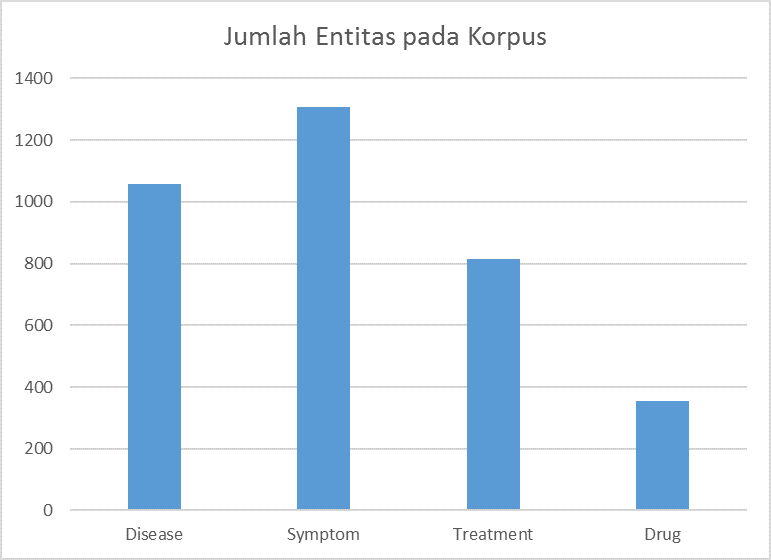
\includegraphics[width=0.85\linewidth]{images/histogramentitaskorpus}
%	\caption{Histogram Jumlah Entitas pada Korpus}
%	\label{fig:korpus}
%\end{figure}
%
%Tabel \ref{diseasecorpus} menunjukkan 39 daftar entitas \textit{disease} teratas yang terdapat di dalam korpus.
%\begin{table}
%	\caption{Tabel Beberapa Entitas \textit{Disease} pada Korpus dan Jumlahnya}
%	\label{diseasecorpus}
%	\resizebox{\textwidth}{!}{%
%		\begin{tabular}{|l|l|l|}
%			\hline
%			asma (20)                                  & isk (20)                         & tbc (18)                             \\ \hline
%			infeksi (17)                               & sinusitis (16)                   & jerawat (15)                         \\ \hline
%			alergi (14)                                & oligomenorea (14)                & maag (12)                            \\ \hline
%			fam (11)                                   & flu (11)                         & kanker serviks (11)                  \\ \hline
%			hiv (11)                                   & penyakit jantung (11)            & varikokel (10)                       \\ \hline
%			wasir (10)                                 & infeksi saluran kemih (9)        & obesitas (9)                         \\ \hline
%			cacar air (9)                              & diabetes (9)                     & albino (9)                           \\ \hline
%			gerd (8)                                   & hepatitis b (8)                  & tth (8)                              \\ \hline
%			liver (8)                                  & sifilis (8)                      & tuberkulosis (7)                     \\ \hline
%			stroke (7)                                 & sakit maag (7)                   & anemia aplastik (7)                  \\ \hline
%			alergi susu sapi (7)                       & hepatitis (7)                    & diare (6)                            \\ \hline
%			scabies (6)                                & kanker otak (6)                  & jengger ayam (6)                     \\ \hline
%			pid (6)                                    & osteoporosis (5)                 & tifus (5)                            \\ \hline
%		\end{tabular}
%	}
%\end{table}
%
%Tabel \ref{symtomcorpus} menunjukkan 39 daftar entitas \textit{symptom} teratas yang terdapat di dalam korpus.
%
%% Please add the following required packages to your document preamble:
%% \usepackage[normalem]{ulem}
%% \useunder{\uline}{\ul}{}
%\begin{table}
%	\caption{Tabel Beberapa Entitas \textit{Symptom} pada Korpus dan Jumlahnya}
%	\label{symtomcorpus}
%	\resizebox{\textwidth}{!}{%
%		\begin{tabular}{|l|l|l|}
%			\hline
%			nyeri (60)                                                     & sakit kepala (51)                                       & demam (50)                                                \\ \hline
%			mual (40)                                                      & gatal (30)                                              & batuk (27)                                                \\ \hline
%			pusing (24)                                                    & muntah (23)                                             & diare (16)                                                \\ \hline
%			keputihan (15)                                                 & nyeri dada (14)                                         & sesak nafas (14)                                          \\ \hline
%			kejang (13)                                                    & keringat dingin (13)                                    & pilek (12)                                                \\ \hline
%			nyeri kepala (10)                                              & stres (10)                                              & stress (10)                                               \\ \hline
%			sesak (8)                                                      & jantung berdebar - debar (7)                            & flu (7)                                                   \\ \hline
%			rasa nyeri (7)                                                 & lemas (7)                                               & kesemutan (7)                                             \\ \hline
%			bersin (6)                                                     & sakit gigi (6)                                          & mimisan (6)                                               \\ \hline
%			nyeri pinggang (6)                                             & depresi (5)                                             & perih (5)                                                 \\ \hline
%			sakit perut (5)                                                & anyang - anyangan (4)                                   & bintilan (4)                                              \\ \hline
%			kram perut (4)                                                 & pingsan (4)                                             & susah tidur (4)                                           \\ \hline
%			rasa gatal (4)                                                 & perubahan mood (4)                                      & kelelahan (4)                                             \\ \hline
%			
%		\end{tabular}
%	}
%\end{table}
%
%
%Tabel \ref{treatmentCorpus} menunjukkan 39 daftar entitas \textit{treatment} teratas yang terdapat di dalam korpus.
%
%% Please add the following required packages to your document preamble:
%% \usepackage{graphicx}
%\begin{table}
%	\caption{Tabel Beberapa Entitas \textit{Treatment} pada Korpus dan Jumlahnya}
%	\label{treatmentCorpus}
%	\resizebox{\textwidth}{!}{%
%		\begin{tabular}{|l|l|l|}
%			\hline
%			operasi (40) & pemeriksaan fisik (34) & terapi (21) \\ \hline
%			usg (15) & pemeriksaan penunjang (11) & tes darah (10) \\ \hline
%			istirahat (9) & pemeriksaan darah (8) & pemeriksaan jantung (7) \\ \hline
%			ct scan (7) & ekg (6) & x - ray (6) \\ \hline
%			foto rontgen (5) & biopsi (5) & imunisasi (5) \\ \hline
%			tes pap (5) & operasi sesar (4) & mri (4) \\ \hline
%			istirahat cukup (4) & kontrasepsi (4) & dinebu (3) \\ \hline
%			tes lbc (3) & minum air putih (3) & rontgen (3) \\ \hline
%			rontgen dada (3) & susu (3) & fisioterapi (3) \\ \hline
%			tes iva (3) & berolahraga (3) & tes penunjang (3) \\ \hline
%			hindari memencet (2) & test pack (2) & terapi obat - obatan (2) \\ \hline
%			makan makanan bergizi (2) & pasang iud (2) & cek darah (2) \\ \hline
%			kompres dingin (2) & tes hpv (2) & gunakan kondom (2) \\ \hline
%		\end{tabular}%
%	}
%\end{table}
%
%Tabel \ref{drugCorpus} menunjukkan 39 daftar entitas \textit{drug} teratas yang terdapat di dalam korpus.
%% Please add the following required packages to your document preamble:
%% \usepackage{graphicx}
%\begin{table}
%	\caption{Tabel Beberapa Entitas \textit{Drug} pada Korpus dan Jumlahnya}
%	\label{drugCorpus}
%	\resizebox{\textwidth}{!}{%
%		\begin{tabular}{|l|l|l|}
%			\hline
%			antibiotik (31) & paracetamol (8) & ibuprofen (7) \\ \hline
%			parasetamol (5) & whey protein (5) & obat tetes mata (5) \\ \hline
%			obat batuk (5) & vitamin c (4) & obat herbal (4) \\ \hline
%			nebulizer (4) & kiranti (4) & salbutamol (4) \\ \hline
%			salep (4) & obat antibiotik (4) & amoxilin (3) \\ \hline
%			metronidazol (3) & obat pelangsing (3) & nitrokaf (3) \\ \hline
%			kortikosteroid (3) & asam mefenamat (3) & tetrahydrolipstatin (3) \\ \hline
%			steroid (3) & ctm (3) & asam valproat (3) \\ \hline
%			rifampicin (3) & obat pereda nyeri (2) & habbatussauda (2) \\ \hline
%			obat depaken (2) & glucovance (2) & obat pereda rasa nyeri (2) \\ \hline
%			obat nyeri (2) & obat penurun panas (2) & probiotik (2) \\ \hline
%			sunblock (2) & obat jerawat (2) & bicrolid (2) \\ \hline
%			plembab (2) & aspirin (2) & acyclovir (2) \\ \hline
%		\end{tabular}%
%	}
%\end{table}
%
%%-----------------------------------------------------------------------------%
%\section{Desain Eksperimen}
%Pada penelitian ini, \saya~melakukan 3 buah skenario utama, yaitu skenario untuk melakukan implementasi dan eksperimen ulang pada \textit{baseline} (penelitian sebelumnya), skenario untuk menguji fitur yang memiliki kontribusi untuk meningkatkan akurasi dari setiap eksperimen dan skenario untuk menguji arsitektur RNNs yang \saya~usulkan. Berikut merupakan skenario yang \saya~rancang dalam penelitian ini:
%\begin{enumerate}
%	\item Skenario 1: Skenario untuk mengimplementasikan ulang eksperimen sebelumnya\\
%	Skenario ini bertujuan untuk mengimplementasikan ulang model yang diusulkan pada penelitian \cite{skripsiKakRadit}, yaitu dengan menggunakan model \textit{Conditional Random Fields} (CRFs). Fitur yang digunakan merupakan fitur yang memberikan hasil terbaik pada penelitian sebelumnya, yaitu fitur kata, fitur kamus, fitur frasa, fitur panjang kata dan fitur kata sebelum. Tujuan dari skenario ini yaitu sebagai \textit{baseline} dan pembanding pada penelitian ini.
%	
%	\item Skenario 2: Skenario untuk menguji fitur\\
%	Skenario ini bertujuan untuk mendapatkan kombinasi fitur terbaik sehingga memberikan akurasi terbaik. \Saya~mencoba masing-masing fitur dengan menggunakan model arsitektur LSTMs 1 layer. Apabila penggunaan fitur memberikan hasil yang lebih dari pada hasil eksperimen sebelumnya, fitur tersebut akan dipertahankan untuk eksperimen yang selanjutnya. Skenario ini memiliki 9 sub-skenario, yaitu:
%	\begin{enumerate}
%		\item Sub-skenario 2.1 Fitur kata
%		\item Sub-skenario 2.2 Fitur kata dan kamus
%		\item Sub-skenario 2.3 Fitur kata, kamus dan \textit{stopword}
%		\item Sub-skenario 2.4 Fitur kata, kamus, \textit{stopword} dan POS-Tag
%		\item Sub-skenario 2.5 Fitur kata, kamus, \textit{stopword}, POS-Tag dan frasa kata
%		\item Sub-skenario 2.5 Fitur kata, kamus, \textit{stopword} dan frasa kata
%		\item Sub-skenario 2.5 Fitur kata, kamus, \textit{stopword}, frasa kata dan kata sebelum
%		\item Sub-skenario 2.5 Fitur kata, kamus, \textit{stopword}, frasa kata, kata sebelum dan kata sesudah
%	\end{enumerate}
%
%	\item Skenario 3: Skenario untuk menguji arsitektur RNNs\\
%	Skenario ini bertujuan untuk melihat pengaruh arsitektur RNNs pada penelitian ini. \Saya~mencoba kedua arsitektur RNNs yang telah diusulkan sebelumnya dengan menggunakan kombinasi fitur terbaik dari eksperimen di skenario pengujian fitur di atas. Pada skenario ini, terdapat 2 sub-skenario, yaitu:
%	\begin{enumerate}
%		\item Sub-skenario 3.1: LSTMs 1 layer
%		\item Sub-skenario 3.2: LSTMs 2 layer multi-\textit{input}
%	\end{enumerate}
%	
%\end{enumerate}
%
%\section{Skenario 1: \textit{Baseline} Eksperimen \cite{skripsiKakRadit}}
%Pada penelitian ini, \saya~mencoba melakukan implementasi ulang penelitian yang dilakukan oleh \cite{skripsiKakRadit}. Data yang digunakan adalah data yang \saya~gunakan dalam penelitian ini supaya perbandingan yang didapatkan \textit{apple-to-apple}. Implementasi dan eksperimen ini bertujuan sebagai \textit{baselaine} eksperimen dan penelitian yang \saya~lakukan. Selain itu, juga untuk mengetahui secara singkat fitur yang diskriminatif dalam melakukan \textit{sequence labeling} pada \mer~ini. Model yang digunakan sama dengan penelitian \cite{skripsiKakRadit}, yaitu CRFs dengan penggunaan fitur kata, fitur kamus, fitur frasa, fitur panjang kata dan fitur kata sebelum.
%
%\subsection{Hasil Eksperimen}
%\textbf{Waktu komputasi}: $ 6093.0 $ detik.
%
%Berikut merupakan hasil implementasi ulang penelitian yang dilakukan oleh \cite{skripsiKakRadit}.
%	
%\begin{table}
%	\centering
%	\caption{Tabel Hasil Eksperimen dari Penelitian \cite{skripsiKakRadit} (\textit{Baseline})}
%	\begin{tabular}{|c|c|c|c|c|}
%		\hline
%							& \textit{Precission} & \f{\f{Recall}} & \f{\f{F-Measure}} \\ \hline
%		\textit{Disease}    & 63.68\%             & 55.45\%        & 59.13\%           \\ \hline
%		\textit{Symptom}    & 61.43\%             & 59.21\%        & 60.18\%           \\ \hline
%		\textit{Treatment}  & 53.10\%             & 45.97\%        & 48.82\%           \\ \hline
%		\textit{Drug}		& 58.99\%             & 44.46\%        & 48.23\%           \\ \hline
%		\textit{\textbf{Overall}}&\textbf{59.03\%}  & \textbf{51.27\%}& \textbf{54.09\%} \\ \hline
%	    \end{tabular}
%\label{table:radit}
%\end{table}
%
%\begin{figure}
%	\centering
%	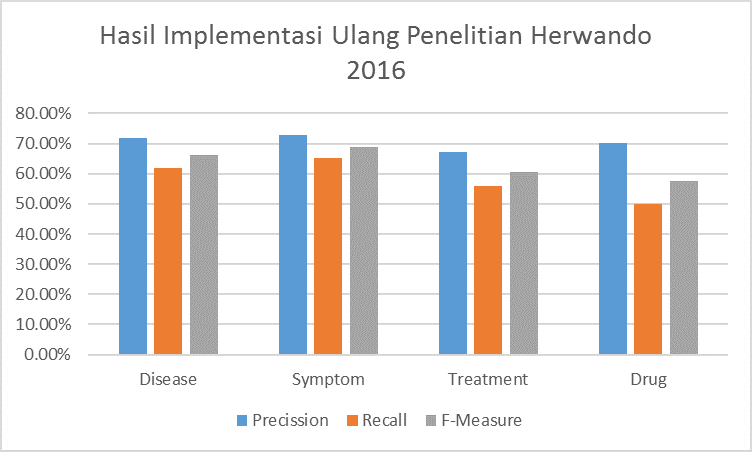
\includegraphics[width=0.85\linewidth]{images/radit}
%	\caption{Histogram Metrik Evaluasi dari Penelitian \cite{skripsiKakRadit} (\textit{Baseline})}
%	\label{fig:radit}
%\end{figure}
%
%
%\section{Skenario 2: Skenario Pengujian Fitur}
%		  
%	\subsection{Eksperimen 2.1: Fitur Kata}
%	%-----------------------------------------------------------------------------%
%	Merujuk pada penelitian \cite{mujiono2016new}, penelitian tersebut bertujuan untuk mendapatkan \textit{non-handcrafted feature}, yaitu fitur kata itu sendiri dengan menggunakan \textit{tools Word Embedding}. Oleh karena itu, \saya~menguji fitur ini untuk mengetahui pengaruhnya pada program \mer~di penelitian ini. 
%	
%	\subsubsection{Hasil Eksperimen}
%	\textbf{Waktu komputasi}: $ 5191.0 $ detik.
%	
%	Tabel \ref{table:ekskata} menampilkan hasil pelabelan otomatis dengan menggunakan fitur kata itu sendiri yang direpresentasikan dengan menggunakan vektor \textit{word embedding}.
%	
%	% Please add the following required packages to your document preamble:
%	% \usepackage{multirow}
%	\begin{table}
%		\centering
%		\caption{Tabel Hasil Eksperimen 2.1 dibandigkan dengan \textit{Baseline}}
%		\begin{tabular}{|l|c|c|c|c|c|c|}
%			\hline
%			\multicolumn{1}{|c|}{\multirow{2}{*}{Entitas}} & \multicolumn{3}{c|}{\textit{Baseline (Herwando 2016)}} & \multicolumn{3}{c|}{Eksperimen 2.1} \\ \cline{2-7} 
%			\multicolumn{1}{|c|}{} & \textit{Precision} & \textit{Recall} & \textit{F-Measure} & \textit{Precision} & \textit{Recall} & \textit{F-Measure} \\ \hline
%			\textit{Disease} & 63.68\% & 55.45\% & 59.13\% & 61.38\% & 60.42\% & 60.37\% \\ \hline
%			\textit{Symptom} & 61.43\% & 59.21\% & 60.18\% & 57.05\% & 56.13\% & 56.19\% \\ \hline
%			\textit{Treatment} & 53.10\% & 45.97\% & 48.82\% & 49.92\% & 47.17\% & 46.96\% \\ \hline
%			\textit{Drug} & 58.99\% & 44.46\% & 48.23\% & 62.86\% & 53.32\% & 57.28\% \\ \hline
%			\textbf{Overall} & \textbf{59.30\%} & \textbf{51.27\%} & \textbf{54.09\%} & \textbf{57.80\%} & \textbf{54.26\%} & \textbf{55.20\%} \\ \hline
%		\end{tabular}
%	\label{table:ekskata}
%	\end{table}
%
%	\begin{figure}
%	  \centering
%	  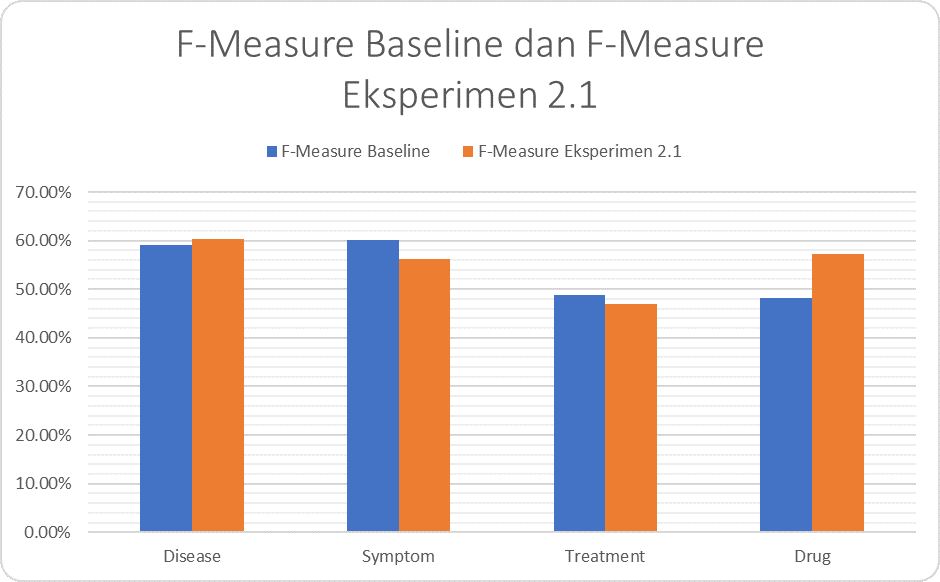
\includegraphics[width=0.85\linewidth]{images/histogram00}
%	  \caption{Histogram Perbandingan \textit{F-measure} \textit{Baseline} dengan Eksperimen 2.1}
%	  \label{fig:ekskata}
%	\end{figure}
%		
%	\subsubsection{Analisis}
%	Pada tabel \ref{table:ekskata}, dapat dilihat bahwa secara umum \textit{recall} dan \textit{F-measure} yang dihasilkan lebih baik dibandingkan dengan \textit{baseline}, walaupun untuk beberapa entitas nilainya lebih rendah (entitas \textit{symptom} dan \textit{treatment}). Selain itu, apabila dilihat pada grafik \ref{fig:ekskata}, secara umum model ini memberikan hasil yang lebih baik pada entitas \textit{disease} dan \textit{drug}. Kemudian rata-rata \textit{F-measure} yang didapatkan yaitu $ 55.20\% $, lebih tinggi dibandingkan \textit{baseline} yang \saya~gunakan yaitu $ 54.09\% $. Hal ini sangat menarik karena hanya dengan penggunaan fitur kata saja, hasil yang diberikan secara umum lebih baik dibandingkan \textit{baseline}.
%	
%	Pada eksperimen ini, ada beberapa entitas masih memiliki nilai \textit{precision, recall} dan \textit{f-measure} lebih kecil apabila dibandingkan dengan hasil yang dicapai \cite{skripsiKakRadit}. Setelah \saya~melakukan analisis terhadap penggunaan penggunaan \textit{tools Word Embedding}, ternyata terdapat 429 kata unik yang tidak terdapat dalam model \textit{word embedding}. Hal ini disebabkan oleh beberapa hal, yaitu:
%	\begin{enumerate}
%		\item Terdapat kata di dalam korpus yang tidak baku atau salah eja\\
%		Korpus yang didapatkan berasal dari forum kesehatan \textit{online} yang bersifat non-formal. Oleh karena itu baik pasien maupun dokter bebas mengutarakan pendapatnya tanpa adanya aturan bahasa formal. Oleh karena itu banyak ditemukan adanya kata yang tidak baku atau salah eja, misalnya:
%		\begin{itemize}
%			\item dllsebaiknya,
%			\item sekatrang,
%			\item infeksiny,
%			\item kliengan.
%		\end{itemize}
%		
%		\item Terdapat istilah sulit yang tidak terkandung di dalam model\\
%		Terdapat beberapa istilah kesehatan pada korpus yang tidak ada di dalam model, hal ini disebabkan karena data untuk \textit{training} model \textit{word embedding} terbatas (model sangat tergantung pada data \textit{training}). Oleh karena terdapat beberapa kata yang tidak terdaftar di dalam model. Contoh beberapa istilah sulit tersebut yaitu:
%		\begin{itemize}
%			\item microdermabrians,
%			\item flixotide,
%			\item bimaflox,
%			\item polysiloxanes,
%			\item scizophrenia.
%		\end{itemize}
%	
%		\item Terdapat kata yang merupakan nama orang\\
%		Adanya kata yang merupakan nama orang tidak bisa dihindari di dalam forum kesehatan \textit{online}. Selain itu, nama orang berbeda untuk setiap orang sehingga sulit mendapatkan vektor kata nama orang tersebut di dalam \textit{word embedding}. Contoh dari kata yang merupakan nama orang di dalam korpus yaitu:
%		\begin{itemize}
%			\item novira,
%			\item risma,
%			\item oktavia,
%			\item sudianto.
%		\end{itemize}
%	\end{enumerate}
%	
%	Dari beberapa kasus di atas, \saya~mengusulkan menambahkan fitur yang memperkaya informasi dari fitur kata itu sendiri, misalnya seperti apakah suatu kata terdapat dalam sebuah kamus kesehatan, informasi POS-Tag atau informasi yang lain. Oleh karena itu, \saya~mencoba menggunakan tambahan fitur lain untuk meningkatkan akurasi pada penelitian ini, yaitu pada sub-eksperimen \ref{eks:subeksdict}.
%	
%	%-----------------------------------------------------------------------------%
%	\subsection{Eksperimen 2.2: Fitur Kata dan Kamus Kesehatan (\textit{Disease, Symptom, Treatment} dan \textit{Drug})}\label{eks:subeksdict}
%	%-----------------------------------------------------------------------------%
%	Pada sub-eksperimen ini, \saya~menggunakan tambahan fitur Kamus Kesehatan karena berdasarkan penelitian \cite{skripsiKakRadit} fitur ini memiliki konribusi untuk menambah akurasi pada sistem \mer. Selain itu, menurut \saya, informasi suatu kata terdapat dalam sebuah kamus kesehatan mungkin akan memberikan kontribusi untuk meningkatkan akurasi. Oleh karena itu, \saya~mencoba untuk menambahkan fitur ini ke dalam model RNNs.
%	
%	\subsubsection{Hasil Eksperimen}
%	\textbf{Waktu komputasi}: $ 5658.0 $ detik.
%	
%	Tabel \ref{table:ekskamus} merupakan tabel hasil eksperimen yang didapatkan dengan menggunakan fitur ini.
%	
%	% Please add the following required packages to your document preamble:
%	% \usepackage{multirow}
%	\begin{table}
%		\centering
%		\caption{Tabel Hasil Eksperimen 2.2 dibandigkan dengan \textit{Baseline}}
%		\label{table:ekskamus}
%		\begin{tabular}{|l|c|c|c|c|c|c|}
%			\hline
%			\multicolumn{1}{|c|}{\multirow{2}{*}{Entitas}} & \multicolumn{3}{c|}{Baseline (Herwando 2016)} & \multicolumn{3}{c|}{Eksperimen 2.2} \\ \cline{2-7} 
%			\multicolumn{1}{|c|}{} & \textit{Precision} & \textit{Recal} & \textit{F-Measure} & \textit{Precision} & \textit{Recal} & \textit{F-Measure} \\ \hline
%			\textit{Disease} & 63.68\% & 55.45\% & 59.13\% & 67.32\% & 61.78\% & 64.10\% \\ \hline
%			\textit{Symptom} & 61.43\% & 59.21\% & 60.18\% & 60.55\% & 55.12\% & 57.41\% \\ \hline
%			\textit{Treatment} & 53.10\% & 45.97\% & 48.82\% & 52.21\% & 44.18\% & 47.02\% \\ \hline
%			\textit{Drug} & 58.99\% & 44.46\% & 48.23\% & 59.42\% & 59.71\% & 57.90\% \\ \hline
%			\textit{\textbf{Overall}} & \textbf{59.30\%} & \textbf{51.27\%} & \textbf{54.09\%} & \textbf{59.88\%} & \textbf{55.20\%} & \textbf{56.61\%} \\ \hline
%		\end{tabular}
%	\end{table}
%	
%	Berikut merupakan grafik yang menunjukkan perbandingan \textit{F-Measure} eksperimen \ref{table:ekskamus} dengan \textit{baseline} dalam bentuk histogram.
%	
%	\begin{figure}
%		\centering
%		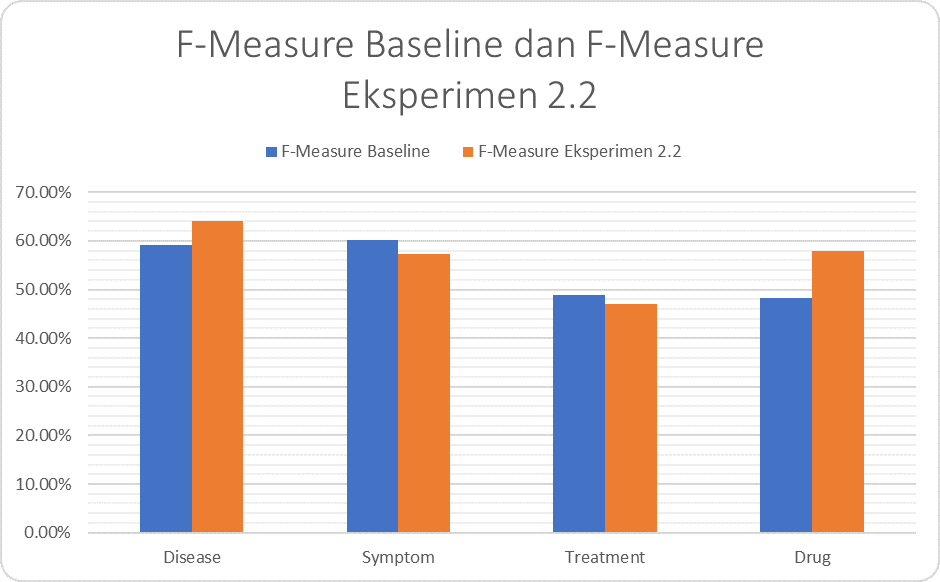
\includegraphics[width=0.85\linewidth]{images/histogram2}
%		\caption{Histogram Perbandingan \textit{F-measure} \textit{Baseline} dengan Eksperimen 2.2}
%		\label{fig:ekskamus}
%	\end{figure}
%
%	\subsubsection{Analisis}
%
%	Dari tabel dan grafik \ref{fig:ekskamus}, didapatkan informasi bahwa dengan menggunakan tambahan fitur kamus kesehatan terlihat bahwa entitas \textit{Disease} mengalami kenaikan nilai \textit{precision}, \textit{recall}, dan \textit{f-measure}. Selain itu, entitas \textit{symptom} dan \textit{tratment} mengalami kenaikan nilai \textit{precision} dan \textit{f-measure}. Entitas \textit{drug} mengalami penurunan pada nilai \textit{precision} namun mengalami kenaikan pada nilai \textit{recall} dan \textit{f-measure}-nya. Secara keseluruhan,  Sedangkan entitas \textit{drug} memiliki \textit{precission} tertinggi, yaitu 62.86\%. Grafik \ref{fig:ekskamus} menunjukkan perbandingan \textit{precision}, \textit{recall} dan \textit{f-measure} untuk masing-masing entitas.
%	
%	Dari analisis yang \saya~lakukan terhadap korpus dan kamus kesehatan, terdapat beberapa entitas pada korpus yang tidak terdapat pada kamus sehingga mengakibatkan kenaikan hasil tidak besar. Hal ini karena terdapat beberapa penyebab, yaitu:
%	\begin{enumerate}
%		\item Ada entitas yang merupakan kombinasi atau gabungan dari entitas lain yang dihubungkan dengan kata penghubung. Hal ini banyak \saya~temukan pada entitas \textit{treatment} dan \textit{symptom}. Contoh dari kasus ini yaitu:
%		\begin{itemize}
%			\item nyeri hebat dibagian ulu hati dan pinggang belakang (gabungan dari "nyeri hebat dibagian ulu hati" dan "nyeri hebat pinggang belakang")
%			\item kondisi fases berampas , kuning , sedikit berlendir (gabungan dari "kondisi fases berampas", "kondisi fases kuning" dan "kondisi fases sedikit berlendir")
%			\item alis atas dan bibir tidak bisa digerakkan (gabungan dari "alis atas tidak bisa digerakkan" dan "bibir tidak bisa digerakkan")
%		\end{itemize}
%		
%		\item Penggunaan kata ganti orang di dalam entitas. Contoh dari kasus ini yaitu:
%		\begin{itemize}
%			\item suara \textbf{saya} hilang
%			\item gusi \textbf{saya} berdarah
%			\item pinggang \textbf{saya} sakit
%		\end{itemize}
%		
%		\item Kesalahan eja pada entitas atau penggunaan kata yang tidak baku, misalnya:
%		\begin{itemize}
%			\item radang paru 2
%			\item butawarna
%			\item jrawatan
%			\item kanker darah setadium 1
%		\end{itemize}
%	\end{enumerate}
%
%	Dibandingkan dengan hasil eksperimen \cite{skripsiKakRadit}, hasil yang dicapai pada eksperimen ini masih lebih rendah pada entitas \textit{symptom} dan \textit{treatment}. Menurut \saya~perlu ada informasi tambahan untuk meningkatkan akurasi. Seperti yang kita ketahui bahwa eksperimen \cite{skripsiKakRadit} tidak hanya menggunakan fitur kata itu sendiri dan kamus kesehatan saja. Oleh karena itu, \saya~mencoba melakukan eksperimen kembali dengan menggunakan tambahan fitur lain pada sub-eksperimen \ref{eks:subekstopword}.
%	
%	%-----------------------------------------------------------------------------%
%	\subsection{Eksperimen 2.3: Fitur Kata, Kamus Kesehatan dan \textit{Stopword}}\label{eks:subekstopword}
%	%-----------------------------------------------------------------------------%
%	Pada sub-eksperimen ini. \saya~mencoba menambahkan informasi lain berupa fitur yang berisi sebuah kata apakah terdapat di dalam kamus \textit{stop word} atau tidak. \Saya~berpendapat bahwa dengan adanya informasi \textit{stop word}, adanya kesalahan suatu kata tidak berentitas yang dilabeli sebagai kata berentitas oleh model dapat dikurangi.
%	
%	\subsubsection{Hasil Eksperimen}
%	\textbf{Waktu komputasi}: $ 6019.5 $ detik.
%	
%	Rangkuman hasil sub-eksperimen ini dapat dilihat di Tabel \ref{table:eksstop} dan Gambar \ref{fig:eksstop}.
%	
%
%	\begin{table}
%		\centering
%		\caption{Tabel Hasil Eksperimen 2.3 dibandigkan dengan \textit{Baseline}}
%		\begin{tabular}{|l|c|c|c|c|c|c|}
%			\hline
%			\multicolumn{1}{|c|}{\multirow{2}{*}{Entitas}} & \multicolumn{3}{c|}{Baseline (Herwando 2016)} & \multicolumn{3}{c|}{Eksperimen 2.3} \\ \cline{2-7} 
%			\multicolumn{1}{|c|}{} & \textit{Precision} & \textit{Recall} & \textit{F-Measure} & \textit{Precision} & \textit{Recall} & \textit{F-Measure} \\ \hline
%			\textit{Disease} & 63.68\% & 55.45\% & 59.13\% & 65.97\% & 59.81\% & 62.28\% \\ \hline
%			\textit{Symptom} & 61.43\% & 59.21\% & 60.18\% & 63.08\% & 55.20\% & 58.68\% \\ \hline
%			\textit{Treatment} & 53.10\% & 45.97\% & 48.82\% & 54.73\% & 46.27\% & 49.69\% \\ \hline
%			\textit{Drug} & 58.99\% & 44.46\% & 48.23\% & 61.88\% & 58.99\% & 59.57\% \\ \hline
%			\textit{\textbf{Overall}} & \textbf{59.30\%} & \textbf{51.27\%} & \textbf{54.09\%} & \textbf{61.42\%} & \textbf{55.07\%} & \textbf{57.56\%} \\ \hline
%		\end{tabular}
%		\label{table:eksstop}
%	\end{table}
%		
%	\begin{figure}
%		\centering
%		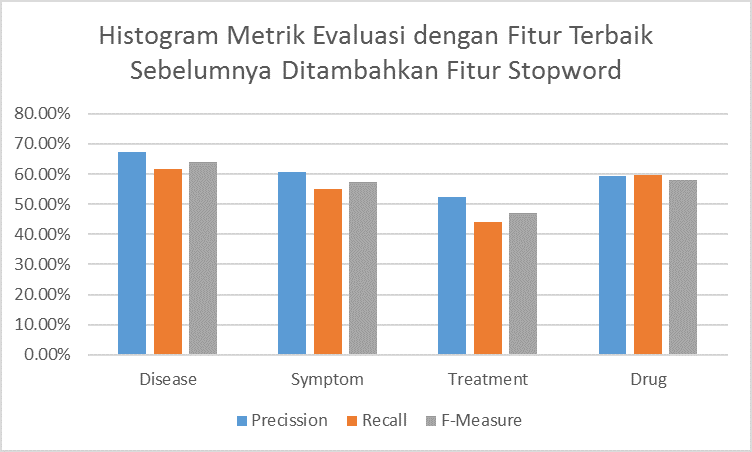
\includegraphics[width=0.85\linewidth]{images/histogram3}
%		\caption{Histogram Perbandingan \textit{F-measure} \textit{Baseline} dengan Eksperimen 2.3}
%		\label{fig:eksstop}
%	\end{figure}
%
%	\subsubsection{Analisis}
%	
%	Dari Tabel \ref{table:eksstop} dan Gambar \ref{fig:eksstop} dapat diamati bahwa secara umum, penggunaan fitur kamus \textit{stop word} dapat meningkatkan \textit{precision, recall,} dan \textit{f-measure}. Untuk lebih detailnya, entitas \textit{disease} mengalami penurunan nilai \textit{precision} dan \textit{f-measure} tetapi mengalami kenaikan nilai \textit{recall}. Entitas \textit{symptom} dan \textit{treatment} mengalami kenaikan untuk nilai \textit{precision, recall} dan \textit{f-measure}. Sedangkan entitas \textit{drug} mengalami kenaikan pada nilai \textit{precission} dan \textit{f-measure} teteapi mengalami penurunan pada nilai \textit{recall}.
%		
%	Pada sub-eksperimen ini, walaupun secara umum akurasi lebih baik dibandingkan dengan sub-eksperimen sebelumnya, hasil sub-eksperimen ini masih lebih rendah pada entitas \textit{treatment} apabila dibandingkan dengan hasil eksperimen \cite{skripsiKakRadit}. Oleh karena \saya~mengusulkan fitur tambahan lain yaitu fitur POS-Tag yang akan dijelaskan pada sub-eksperimen \ref{eks:subekspostag}.
%	
%	%-----------------------------------------------------------------------------%
%	\subsection{Eksperimen 2.4: Fitur Kata, Kamus Kesehatan, \textit{Stopword} dan POS-Tag}\label{eks:subekspostag}
%	%-----------------------------------------------------------------------------%
%	Pada sub-eksperimen ini, \saya~menambahkan informasi baru pada \textit{resource} yang akan digunakan untuk \textit{training} model yang berupa fitur POS-Tag. Sebelumnya fitur ini telah digunakan pada penelitian \cite{abacha2011medical} pada dokumen berbahasa Inggris dan memberikan kontribusi meningkatkan akurasi dari model \mer~yang dibangun. Oleh karena itu pada eksperimen ini \saya~mencoba menggunakan fitur tersebut dan ingin mengetahui apakah fitur POS-Tag memiliki kontribusi untuk meningkatkan akurasi pada \mer~dengan dokumen berbahasa Indonesia. 
%	
%	\subsubsection{Hasil Eksperimen}
%	\textbf{Waktu komputasi}: $ 6952.0 $ detik.
%	
%	Rangkuman hasil sub-eksperimen ini dapat dilihat pada Tabel \ref{table:owndict4} dan Gambar \ref{fig:owndict4}.
%	
%	\begin{table}
%		\centering
%		\caption{Tabel Hasil Eksperimen 2.4 dibandigkan dengan \textit{Baseline}}
%		\begin{tabular}{|l|c|c|c|c|c|c|}
%			\hline
%			\multicolumn{1}{|c|}{\multirow{2}{*}{Entitas}} & \multicolumn{3}{c|}{Baseline (Herwando 2016)} & \multicolumn{3}{c|}{Eksperimen 2.4} \\ \cline{2-7} 
%			\multicolumn{1}{|c|}{} & \textit{Precision} & \textit{Recall} & \textit{F-Measure} & \textit{Precision} & \textit{Recall} & \textit{F-Measure} \\ \hline
%			\textit{Disease} & 63.68\% & 55.45\% & 59.13\% & 69.10\% & 58.67\% & 63.22\% \\ \hline
%			\textit{Symptom} & 61.43\% & 59.21\% & 60.18\% & 61.09\% & 54.43\% & 57.00\% \\ \hline
%			\textit{Treatment} & 53.10\% & 45.97\% & 48.82\% & 59.73\% & 44.10\% & 49.87\% \\ \hline
%			\textit{Drug} & 58.99\% & 44.46\% & 48.23\% & 62.00\% & 55.74\% & 57.87\% \\ \hline
%			\textit{\textbf{Overall}} & \textbf{59.30\%} & \textbf{51.27\%} & \textbf{54.09\%} & \textbf{62.98\%} & \textbf{53.24\%} & \textbf{56.99\%} \\ \hline
%		\end{tabular}
%		\label{table:owndict4}
%	\end{table}
%	
%	\begin{figure}
%		\centering
%		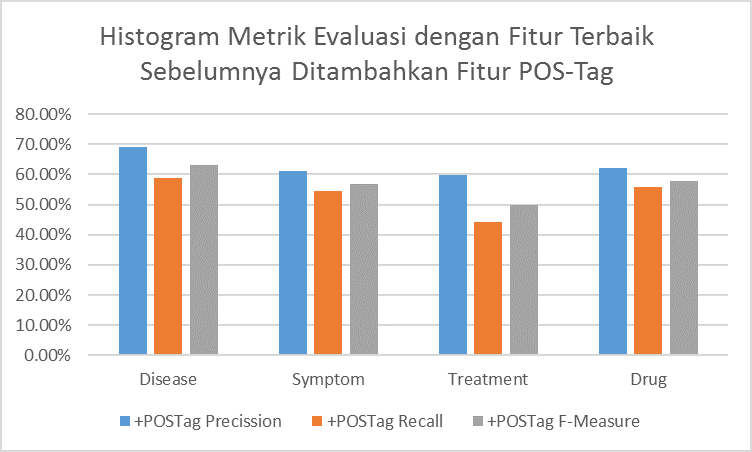
\includegraphics[width=0.85\linewidth]{images/histogram4}
%		\caption{Histogram Perbandingan \textit{F-measure} \textit{Baseline} dengan Eksperimen 2.4}
%		\label{fig:owndict4}
%	\end{figure}
%	
%	\subsubsection{Analisis}
%	Dari tabel dan grafik di atas, entitas \textit{disease} dan \textit{treatment} memiliki nilai \textit{precision} dan \textit{f-measure} yang meningkat, tetapi dengan nilai \textit{recall} yang turun. Untuk entitas \textit{symptom}, nilai \textit{precision, recall}, dan \textit{f-measure} mengalami penurunan. Sedangkan entitas \textit{drug} mengalami kenaikan hanya pada \textit{precision}-nya saja.
%	
%	Hasil dari penggunaan fitur ini kurang baik, karena beberapa hal, yaitu:
%	\begin{enumerate}
%		\item Tag yang dihasilkan tidak konsisten. Pada beberapa entitas, terkadang suatu kata mendapatkan tag "A", namun di entitas yang lain untuk kata yang sama mendapatkan tag yang berbeda. Contoh dari kasus ini yaitu:
%		\begin{itemize}
%			\item "antibiotik" memiliki tag "vb", sedangkan pada entitas lain "antibiotik" memiliki tag "NN"
%			\item "sakit kepala" memiliki beberapa tag pada entitas berbeda, yaitu "CD NN", "JJ NN", dan "NN NN"
%			\item "nyeri" memiliki beberapa tag pada entitas berbeda, yaitu "NN", "VB", "IN", "WH", dan "IN".
%		\end{itemize}
%		\item Tidak ada perbedaan tag antara kata berentitas dengan tidak, misalnya nama orang mendapatkan tag "NN" (intan\_NN lusia\_NN), namun nama penyakit juga mendapatkan tag "NN" (Kanker\_NN Otak\_NN).
%		\item Model POS-Tagger yang digunakan merupakan model untuk kalimat dengan topik umum, tidak dikhususkan pada topik kesehatan.
%	\end{enumerate}
%	
%	Oleh karena itu pada sub-eksperimen selanjutnya, \saya~mencoba menambahkan fitur lain yang lebih spesifik dibandingkan dengan fitur POS-Tag, yaitu fitur Frasa Kata. Penjelasan lebih lanjut akan dibahas pada sub-eksperimen \ref{eks:subeksfrasa}.
%	
%	%-----------------------------------------------------------------------------%
%	\subsection{Eksperimen 2.5: Fitur Kata, Kamus Kesehatan, \textit{Stopword}, POS-Tag dan Frasa Kata}\label{eks:subeksfrasa}
%	%-----------------------------------------------------------------------------%
%	Pada sub-eksperimen ini \saya~menambahkan fitur baru yaitu fitur Frasa Kata. Seperti yang telah dijelaskan pada Bab 3, entitas \textit{symptom} dan \textit{treatment} diharapkan akan lebih mudah dikenali karena pada umumnya merupakan frasa kata kerja. Sedangkan entitas \textit{disease} dan \textit{drug} diharapkan juga akan lebih mudah dikenali karena pada umumnya merupakan frasa kata benda.
%	
%	\subsubsection{Hasil Eksperimen}
%	\textbf{Waktu komputasi}: $ 7528.5 $ detik.
%	
%	Rangkuman hasil sub-eksperimen ini dapat dilihat pada Tabel \ref{table:owndict4} dan Gambar \ref{fig:owndict4}.
%	
%	\begin{table}
%		\centering
%		\caption{Tabel Hasil Eksperimen 2.5 dibandigkan dengan \textit{Baseline}}
%		\begin{tabular}{|l|c|c|c|c|c|c|}
%			\hline
%			\multicolumn{1}{|c|}{\multirow{2}{*}{Entitas}} & \multicolumn{3}{c|}{Baseline (Herwando 2016)} & \multicolumn{3}{c|}{Eksperimen 2.5} \\ \cline{2-7} 
%			\multicolumn{1}{|c|}{} & \textit{Precision} & \textit{Recall} & \textit{F-Measure} & \textit{Precision} & \textit{Recall} & \textit{F-Measure} \\ \hline
%			\textit{Disease} & 63.68\% & 55.45\% & 59.13\% & 67.49\% & 61.56\% & 63.81\% \\ \hline
%			\textit{Symptom} & 61.43\% & 59.21\% & 60.18\% & 62.89\% & 52.27\% & 56.72\% \\ \hline
%			\textit{Treatment} & 53.10\% & 45.97\% & 48.82\% & 54.87\% & 44.92\% & 49.06\% \\ \hline
%			\textit{Drug} & 58.99\% & 44.46\% & 48.23\% & 59.77\% & 53.37\% & 55.66\% \\ \hline
%			\textit{\textbf{Overall}} & \textbf{59.30\%} & \textbf{51.27\%} & \textbf{54.09\%} & \textbf{61.26\%} & \textbf{53.03\%} & \textbf{56.31\%} \\ \hline
%		\end{tabular}
%		\label{table:owndict5}
%	\end{table}
%
%	\begin{figure}
%		\centering
%		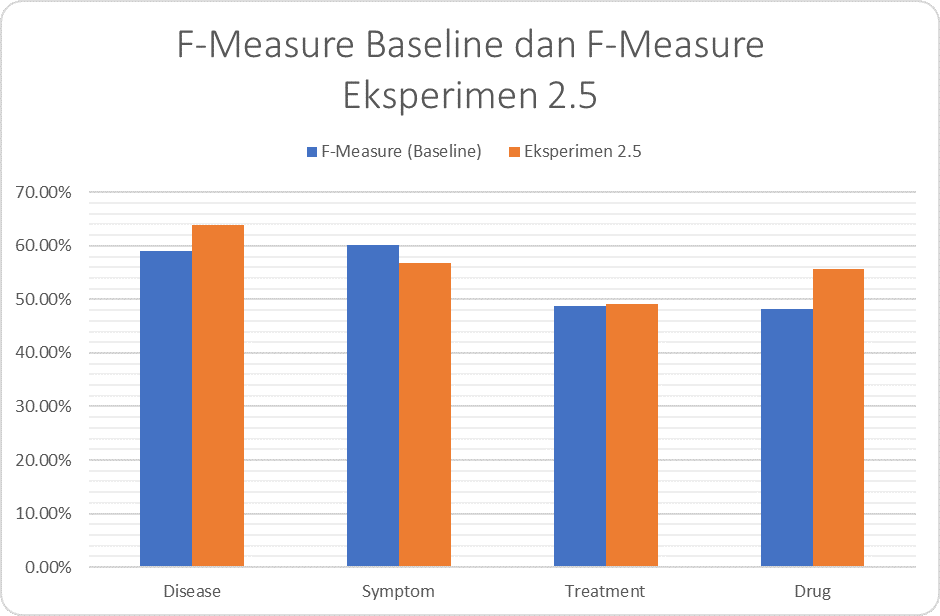
\includegraphics[width=0.85\linewidth]{images/histogram5}
%		\caption{Histogram Perbandingan \textit{F-measure} \textit{Baseline} dengan Eksperimen 2.5}
%		\label{fig:owndict5}
%	\end{figure}
%
%	\subsubsection{Analisis}
%	Dari tabel dan grafik di atas, entitas \textit{drug} mengalami penurunan untuk nilai \textit{precission, recall} dan \textit{f-measure}. Selain itu, entitas \textit{disease} mengalami penurunan pada nilai \textit{precission} tetapi mengalami kenaikan pada nilai \textit{recall} dan \textit{f-measure}. Entitas \textit{symptom} mengalami kenaikan pada nilai \textit{precision} tetapi mengalami penurunan pada nilai \textit{recall} dan \textit{f-measure}. Sedangkan pada entitas \textit{treatment}, terjadi kenaikan nilai \textit{recall} tetapi nilai \textit{precision} dan \textit{f-measure} mengalami penurunan. 
%	
%	Dari korpus yang \saya~miliki, berikut merupakan informasi statistik dari penggunaan fitur frasa kata kerja:
%	\begin{enumerate}
%		\item Untuk entitas \textit{disease}, sebanyak 442 entitas merupakan frasa kata benda, 31 entitas merupakan bagian dari frasa kata benda dan 583 entitas bukan merupakan frasa.
%		\item Untuk entitas \textit{symptom}, sebanyak 486 entitas merupakan frasa kata benda, 194 entitas merupakan bagian dari frasa kata benda dan 626 entitas bukan merupakan frasa.
%		\item Untuk entitas \textit{treatment}, sebanyak 338 entitas merupakan frasa kata benda, 76 entitas merupakan bagian dari frasa kata benda dan 401 entitas bukan merupakan frasa.
%		\item Untuk entitas \textit{drug}, sebanyak 152 entitas merupakan frasa kata benda, 8 entitas merupakan bagian dari frasa kata benda dan 194 entitas bukan merupakan frasa.
%	\end{enumerate}
%
%	Sedangkan berikut merupakan informasi statistik dari penggunaan fitur frasa kata benda:
%	\begin{enumerate}
%		\item Untuk entitas \textit{disease}, sebanyak 943 entitas merupakan frasa kata benda, 43 entitas merupakan bagian dari frasa kata benda dan 70 entitas bukan merupakan frasa.
%		\item Untuk entitas \textit{symptom}, sebanyak 842 entitas merupakan frasa kata benda, 363 entitas merupakan bagian dari frasa kata benda dan 101 entitas bukan merupakan frasa.
%		\item Untuk entitas \textit{treatment}, sebanyak 561 entitas merupakan frasa kata benda, 201 entitas merupakan bagian dari frasa kata benda dan 53 entitas bukan merupakan frasa.
%		\item Untuk entitas \textit{drug}, sebanyak 318 entitas merupakan frasa kata benda, 14 entitas merupakan bagian dari frasa kata benda dan 22  entitas bukan merupakan frasa.
%	\end{enumerate}
%	
%	Dari 2 informasi di atas, dapat diambil informasi bahwa sebagian besar entitas \textit{disease} dan \textit{drug} merupakan frasa kata benda dan entitas \textit{symptom} dan \textit{treatment} merupakan frasa kata kerja. Hal ini menjadi seharusnya menjadi informasi pembeda dengan kata yang bukan merupakan entitas. Namun apabila dilihat dari hasil eksperimen ini, performa penggunaan fitur ini tidak terlalu bagus atau bahkan turun di entitas \textit{disease} dan \textit{symptom} tersebut. \Saya~berpendapat hal ini terjadi karena penggunaan fitur ini sudah cukup mewakili informasi fitur POS-Tag, akrena untuk menentukan suatu kata atau kumpulan kata merupakan frasa adalah dengan menggunakan POS-Tag. Selain itu, pada fitur POS-Tag, tidak ada perbedaan antara kata yang merupakan frasa maupun kata yang bukan frasa. Padahal, mayoritas entitas seperti yang telah dijelaskan di atas merupakan frasa. Oleh karena itu, pada sub-eksperimen \ref{eks:subeksminpostag}, penulis menghilangkan fitur POS-Tag dan tetap mempertahankan fitur frasa kata untuk mengetahui hal tersebut. 
%	
%	%-----------------------------------------------------------------------------%
%	\subsection{Eksperimen 2.6: Fitur Kata, Kamus Kesehatan, \textit{Stopword} dan Frasa Kata}\label{eks:subeksminpostag}
%	%-----------------------------------------------------------------------------%
%	Pada sub-eksperimen ini \saya~menghilangkan fitur POS-Tag berdasarkan hasil dan analisis pada sub-eksperimen \ref{eks:subeksfrasa}.
%	
%	\subsubsection{Hasil Eksperimen}
%	\textbf{Waktu komputasi}: $ 6636.5 $ detik.
%	
%	Rangkuman hasil sub-eksperimen ini dapat dilihat pada Tabel \ref{table:owndict6} dan Gambar \ref{fig:owndict6}.
%	\begin{table}
%		\centering
%		\caption{Tabel Hasil Eksperimen 2.6 dibandigkan dengan \textit{Baseline}}
%		\begin{tabular}{|l|c|c|c|c|c|c|}
%			\hline
%			\multicolumn{1}{|c|}{\multirow{2}{*}{Entitas}} & \multicolumn{3}{c|}{Baseline (Herwando 2016)} & \multicolumn{3}{c|}{Eksperimen 2.6} \\ \cline{2-7} 
%			\multicolumn{1}{|c|}{} & \textit{Precision} & \textit{Recall} & \textit{F-Measure} & \textit{Precision} & \textit{Recall} & \textit{F-Measure} \\ \hline
%			\textit{Disease} & 63.68\% & 55.45\% & 59.13\% & 68.67\% & 61.80\% & 64.78\% \\ \hline
%			\textit{Symptom} & 61.43\% & 59.21\% & 60.18\% & 63.79\% & 56.10\% & 59.23\% \\ \hline
%			\textit{Treatment} & 53.10\% & 45.97\% & 48.82\% & 54.47\% & 46.72\% & 49.58\% \\ \hline
%			\textit{Drug} & 58.99\% & 44.46\% & 48.23\% & 60.08\% & 56.70\% & 57.00\% \\ \hline
%			\textit{\textbf{Overall}} & \textbf{59.30\%} & \textbf{51.27\%} & \textbf{54.09\%} & \textbf{61.75\%} & \textbf{55.33\%} & \textbf{57.65\%} \\ \hline
%		\end{tabular}
%		\label{table:owndict6}
%	\end{table}
%	
%	\begin{figure}
%		\centering
%		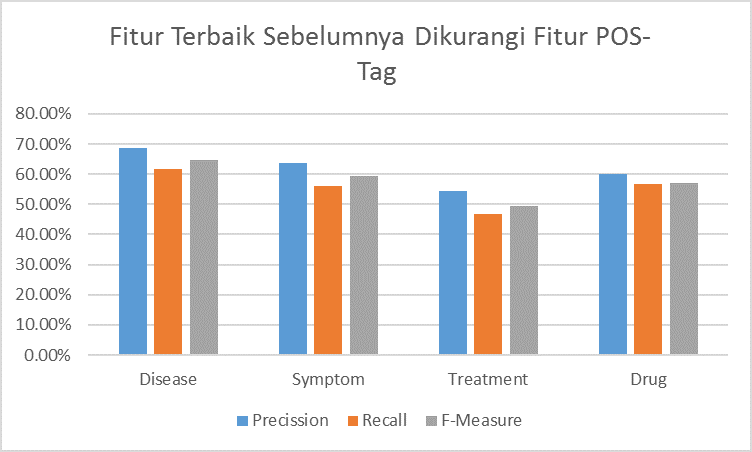
\includegraphics[width=0.85\linewidth]{images/histogram6}
%		\caption{Histogram Perbandingan \textit{F-measure} \textit{Baseline} dengan Eksperimen 2.4, 2.5 dan 2.6}
%		\label{fig:owndict6}
%	\end{figure}
%	
%	\subsubsection{Analisis}
%	Dari Tabel \ref{table:owndict6} dan Gambar \ref{fig:owndict6}, terlihat bahwa semua entitas (\textit{disease, symptom, treatment,}) dan \textit{drug} mengalami kenaikan pada nilai \textit{precision, recall,} dan \textit{f-measure}. Seperti yang telah dijelaskan pada sub-eksperimen \ref{eks:subeksfrasa}, penggabungan fitur POS-Tag dan frasa akan memberikan hasil yang lebih rendah. Oleh karena itu, sebaiknya fitur POS-Tag tidak digabung dengan fitur frasa.
%	
%	Untuk mempermudah dalam membandingkan hasil eksperimen 2.4, 2.5 dan 2.6, \saya~menyajikan grafik \ref{fig:owndict6} untuk membandingkan nilai \textit{F-Measure} pada masing-masing eksperimen. Dapat dilihat bahwa apabila fitur POS-Tag dan Frasa digunakan secara bersama-sama, hasil yang diberikan lebih rendah apabila kedua fitur tersebut dipisah. Namun, apabila dengan menggunakan fitur POS-Tag tanpa Frasa, hasil pada entitas \textit{treatment} dan \textit{drug} lebih bagus. Sedangkan apabila dengan menggunakan fitur Frasa tanpa POS-Tag, hasil pada entitas \textit{disease} dan \textit{symptom} lebih baik. Oleh karena itu \saya~memilih salah satu dari kedua fitur tersebut. Apabila dilihat dari rata-rata \textit{F-Measure}, penggunaan fitur Frasa tanpa POS-Tag memberikan hasil yang paling tinggi ($ 57.65\% $) apabila dibandingkan dengan penggunaan fitur POS-Tag tanpa Frasa ($ 56.99\% $). Oleh karena itu, \saya~mempertahankan fitur Frasa dan tidak menggunakan fitur POS-tag pada eksperimen selanjutnya.
%	
%	Walaupun pada sub-eksperimen ini hasil yang dicapai lebih baik dari sub-eksperimen sebelumnya, hasilnya tetap lebih rendah dari hasil eksperimen \cite{skripsiKakRadit} pada nilai \textit{recall} dan \textit{f-measure} pada entitas \textit{symptom}. Oleh karena itu \saya~mencoba fitur yang lain, yaitu fitur Kata Sebelum. Untuk penjelasan lebih lanjut akan dibahas pada sub-eksperimen \ref{eks:subekswbef1}.
%	
%	%-----------------------------------------------------------------------------%
%	\subsection{Eksperimen 2.7: Fitur Kata, Kamus Kesehatan, \textit{Stopword}, Frasa Kata dan Kata Sebelum}\label{eks:subekswbef1}
%	%-----------------------------------------------------------------------------%
%	Pada sub-eksperimen ini \saya~menambahkan fitur baru yaitu fitur 1 kata sebelum. Fitur ini digunakan pada penelitian \cite{skripsiKakRadit} yang juga berkontribusi memberikan hasil terbaik pada penelitiannya. Menurut \saya, ada beberapa entitas yang akan lebih mudah diketahui apabila diketahui kata sebelumnya. Misalnya kata "masuk angin", apabila hanya diberikan informasi kata "angin" tanpa kata "masuk", akan lebih sulit menentukan kata tersebut bagian dari suatu entitas \textit{disease} atau bukan. Oleh karena itu, pada sub-eksperimen ini \saya~mencoba menambahkan fitur tersebut.
%	
%	\subsubsection{Hasil Eksperimen}
%	\textbf{Waktu komputasi}: $ 9275.5 $ detik.
%	
%	Rangkuman hasil sub-eksperimen ini dapat dilihat pada Tabel \ref{table:owndict7} dan Gambar \ref{fig:owndict7}.
%	
%	\begin{table}
%		\centering
%		\caption{Tabel Hasil Eksperimen 2.7 dibandigkan dengan \textit{Baseline}}
%		\begin{tabular}{|l|c|c|c|c|c|c|}
%			\hline
%			\multicolumn{1}{|c|}{\multirow{2}{*}{Entitas}} & \multicolumn{3}{c|}{Baseline (Herwando 2016)} & \multicolumn{3}{c|}{Eksperimen 2.7} \\ \cline{2-7} 
%			\multicolumn{1}{|c|}{} & \textit{Precision} & \textit{Recall} & \textit{F-Measure} & \textit{Precision} & \textit{Recall} & \textit{F-Measure} \\ \hline
%			\textit{Disease} & 63.68\% & 55.45\% & 59.13\% & 69.49\% & 61.60\% & 64.68\% \\ \hline
%			\textit{Symptom} & 61.43\% & 59.21\% & 60.18\% & 64.78\% & 57.15\% & 60.23\% \\ \hline
%			\textit{Treatment} & 53.10\% & 45.97\% & 48.82\% & 56.58\% & 44.71\% & 49.54\% \\ \hline
%			\textit{Drug} & 58.99\% & 44.46\% & 48.23\% & 62.22\% & 57.28\% & 58.76\% \\ \hline
%			\textit{\textbf{Overall}} & \textbf{59.30\%} & \textbf{51.27\%} & \textbf{54.09\%} & \textbf{63.27\%} & \textbf{55.19\%} & \textbf{58.30\%} \\ \hline
%		\end{tabular}
%		\label{table:owndict7}
%	\end{table}
%	
%	\begin{figure}
%		\centering
%		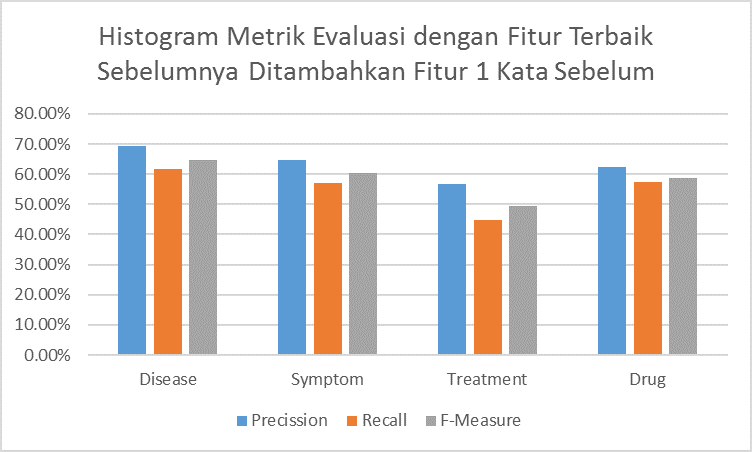
\includegraphics[width=0.85\linewidth]{images/histogram7}
%		\caption{Histogram Perbandingan \textit{F-measure} \textit{Baseline} dengan Eksperimen 2.7}
%		\label{fig:owndict7}
%	\end{figure}
%	
%	\subsubsection{Analisis}
%	Melihat pada Tabel \ref{table:owndict7} dan Gambar \ref{fig:owndict7}, dapat diketahui bahwa entitas \textit{disease} dan \textit{treatment} mengalami kenaikan pada nilai \textit{precission}, tetapi mengalami penurunan pada nilai \textit{recall} dan \textit{f-measure}. Sedangkan entitas \textit{symptom} dan \textit{drug} mengalami kenaikan pada nilai \textit{precision, recall,} dan \textit{f-measure}.
%	
%	Seperti pada penelitian \cite{skripsiKakRadit}, fitur ini berhasil meningkatkan performa dari beberapa entitas, karena fitur ini memberikan informasi tambahan kata sebelumnya, misalnya:
%	\begin{itemize}
%		\item "penyakit", "penderita", "mengalami" dan "mengalami" dapat memberikan informasi mengenai entitas \textit{disease}
%		\item "mengandung", "minum", "pemberian", "obat", "menggunakan" dapat memberikan informasi mengenai entitas \textit{drug}
%		\item "dengan", "melakukan", "dilakukan" dapat memberikan informasi mengenai entitas \textit{treatment}
%		\item "mengalami", "disertai", "sering", "keluhan", "penyebab" dapat memberikan informasi mengenai entitas \textit{symptom}
%	\end{itemize}
%	
%	Hasil sub-eksperimen ini masih lebih rendah dibandingkan dengan hasil eksperimen \cite{skripsiKakRadit} pada \textit{recall} dan \textit{f-measure} entitas \textit{treatment}. Oleh karena itu, \saya~mencoba menambahkan fitur yang lain yaitu fitur 1 Kata sesudah, yang akan dibahas lebih lanjut pada sub-eksperimen \ref{eks:subekswaf1}.
%	
%	
%	%-----------------------------------------------------------------------------%
%	\subsection{Eksperimen 2.8: Fitur Kata, Kamus Kesehatan, \textit{Stopword}, Frasa Kata, Kata Sebelum dan Kata Sesudah}\label{eks:subekswaf1}
%	%-----------------------------------------------------------------------------%
%	Pada sub-eksperimen ini \saya~menambahkan fitur lain yaitu fitur 1 Kata Setelah. Hal ini karena ada beberapa kasus yang mana apabila suatu kata merupakan sebuah entitas, akan lebih mudah dikenali apabila melihat kata atau konteks setelahnya. Sama seperti contoh pada fitur 1 kata sebelum, misal diberikan kata "masuk angin", apabila hanya diberikan informasi "masuk" tanpa "angin", akan lebih sulit mengenali apakah kata tersebut termasuk entitas \textit{disease} atau bukan. Selain itu, fitur ini juga dapat membedakan kata berentitas dengan kata yang bukan, misalnya kata "masuk angin" dengan "masuk rumah". Apabila informasi pada saat tersebut hanya diberikan kata "masuk" saja tanpa kata setelahnya, akan lebih sulit mengenali kata tersebut termasuk kata berentitas atau bukan.
%	
%	\subsubsection{Hasil Eksperimen}
%	\textbf{Waktu komputasi}: $ 14031.5 $ detik.
%	
%	Rangkuman hasil sub-eksperimen ini dapat dilihat pada Tabel \ref{table:owndict8} dan Gambar \ref{fig:owndict8}.
%	
%	\begin{table}
%		\centering
%		\caption{Tabel Hasil Eksperimen 2.8 dibandigkan dengan \textit{Baseline}}
%		\begin{tabular}{|l|c|c|c|c|c|c|}
%			\hline
%			\multicolumn{1}{|c|}{\multirow{2}{*}{Entitas}} & \multicolumn{3}{c|}{Baseline (Herwando 2016)} & \multicolumn{3}{c|}{Eksperimen 2.7} \\ \cline{2-7} 
%			\multicolumn{1}{|c|}{} & \textit{Precision} & \textit{Recall} & \textit{F-Measure} & \textit{Precision} & \textit{Recall} & \textit{F-Measure} \\ \hline
%			\textit{Disease} & 63.68\% & 55.45\% & 59.13\% & 70.68\% & 66.18\% & 68.17\% \\ \hline
%			\textit{Symptom} & 61.43\% & 59.21\% & 60.18\% & 64.16\% & 59.55\% & 60.23\% \\ \hline
%			\textit{Treatment} & 53.10\% & 45.97\% & 48.82\% & 61.02\% & 51.13\% & 54.03\% \\ \hline
%			\textit{Drug} & 58.99\% & 44.46\% & 48.23\% & 70.85.\% & 70.33\% & 69.82\% \\ \hline
%			\textit{\textbf{Overall}} & \textbf{59.30\%} & \textbf{51.27\%} & \textbf{54.09\%} & \textbf{65.29\%} & \textbf{61.80\%} & \textbf{63.06\%} \\ \hline
%		\end{tabular}
%		\label{table:owndict8}
%	\end{table}
%	
%	\begin{figure}
%		\centering
%		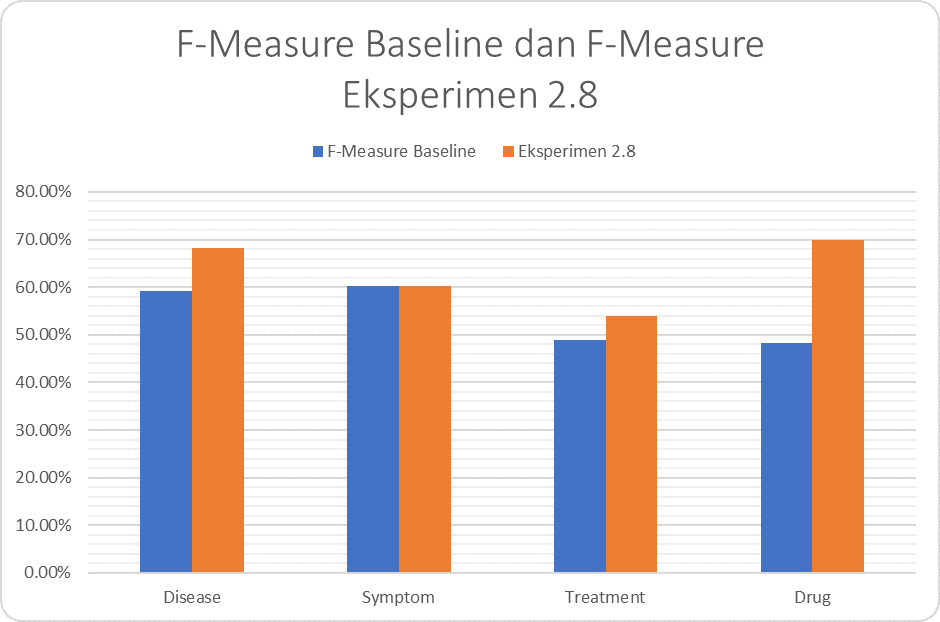
\includegraphics[width=0.85\linewidth]{images/histogram8}
%		\caption{Histogram Perbandingan \textit{F-measure} \textit{Baseline} dengan Eksperimen 2.8}
%		\label{fig:owndict8}
%	\end{figure}
%	
%	\subsubsection{Analisis}
%	Melihat pada Tabel \ref{table:owndict8} dan Gambar \ref{fig:owndict8}, dapat diketahui bahwa hanya entitas \textit{symptom} yang mengalami penurunan nilai pada \textit{precision}, tetapi nilai \textit{recall} dan \textit{f-measure}-nya naik. Sedangkan entitas lain mengalami kenaikan pada nilai \textit{precision, recall} dan \textit{f-measure}. Oleh karena itu, setelah \saya~mencoba kemungkinan fitur yang memberikan kontribusi dalam penelitian ini, \saya~mencoba arsitektur untuk model RNNs yang lain. Penjelasan lebih lanjut akan dibahas pada eksperimen \ref{eks:eks2}.
%	
%	
%	
%  %-----------------------------------------------------------------------------%
%  
%  
%\section{Skenario 3: Skenario Pengujian Arsitektur RNNs}\label{eks:eks2}
%    
%    Pada eksperimen ini, \saya~mencoba dua buah arsitektur RNNs yang telah \saya~usulkan pada Bab 3 yaitu RNNs dengan 1 layer dan RNNs dengan 2 layer. Fitur yang digunakan dalam pengujian ini yaitu kombinasi fitur yang menghasilkan akurasi terbaik pada eksperimen pertama, yaitu fitur kata itu sendiri, kamus kesehatan, \textit{stop word}, frasa kata, 1 kata sebelum dan 1 kata sesudah.
%    
%    \subsection{Eksperimen 3.1: Menguji Arsitektur LSTMs 1 Layer}\label{eks2:subeksrnn1}
%    %-----------------------------------------------------------------------------%
%    Pada sub-eksperimen ini, \saya~menggunakan struktur RNNs yang mana semua fitur digabung menjadi satu dalam sebuah \textit{timestep}.
%    Artinya fitur-fitur yang berbeda tersebut akan digabung atau di-\textit{concat} menjadi sebuah vektor yang akan menjadi \textit{input} bagi LSTMs ini. LSTMs inilah yang digunakan pada eksperimen pertama, sehingga hasilnya sama dengan sub-eksperimen \ref{eks:subekswaf1}.
%    
%    \subsubsection{Hasil Eksperimen}
%    \textbf{Waktu komputasi}: $ 14031.5 $ detik.
%    
%    \begin{table}
%    	\centering
%    	\caption{Tabel Hasil Eksperimen 3.1 dibandigkan dengan \textit{Baseline}}
%    	\begin{tabular}{|l|c|c|c|c|c|c|}
%    		\hline
%    		\multicolumn{1}{|c|}{\multirow{2}{*}{Entitas}} & \multicolumn{3}{c|}{Baseline (Herwando 2016)} & \multicolumn{3}{c|}{Eksperimen 2.7} \\ \cline{2-7} 
%    		\multicolumn{1}{|c|}{} & \textit{Precision} & \textit{Recall} & \textit{F-Measure} & \textit{Precision} & \textit{Recall} & \textit{F-Measure} \\ \hline
%    		\textit{Disease} & 63.68\% & 55.45\% & 59.13\% & 70.68\% & 66.18\% & 68.17\% \\ \hline
%    		\textit{Symptom} & 61.43\% & 59.21\% & 60.18\% & 64.16\% & 59.55\% & 60.23\% \\ \hline
%    		\textit{Treatment} & 53.10\% & 45.97\% & 48.82\% & 61.02\% & 51.13\% & 54.03\% \\ \hline
%    		\textit{Drug} & 58.99\% & 44.46\% & 48.23\% & 70.85.\% & 70.33\% & 69.82\% \\ \hline
%    		\textit{\textbf{Overall}} & \textbf{59.30\%} & \textbf{51.27\%} & \textbf{54.09\%} & \textbf{65.29\%} & \textbf{61.80\%} & \textbf{63.06\%} \\ \hline
%    	\end{tabular}
%    	\label{table:owndict9}
%    \end{table}
%    
%    \begin{figure}
%    	\centering
%    	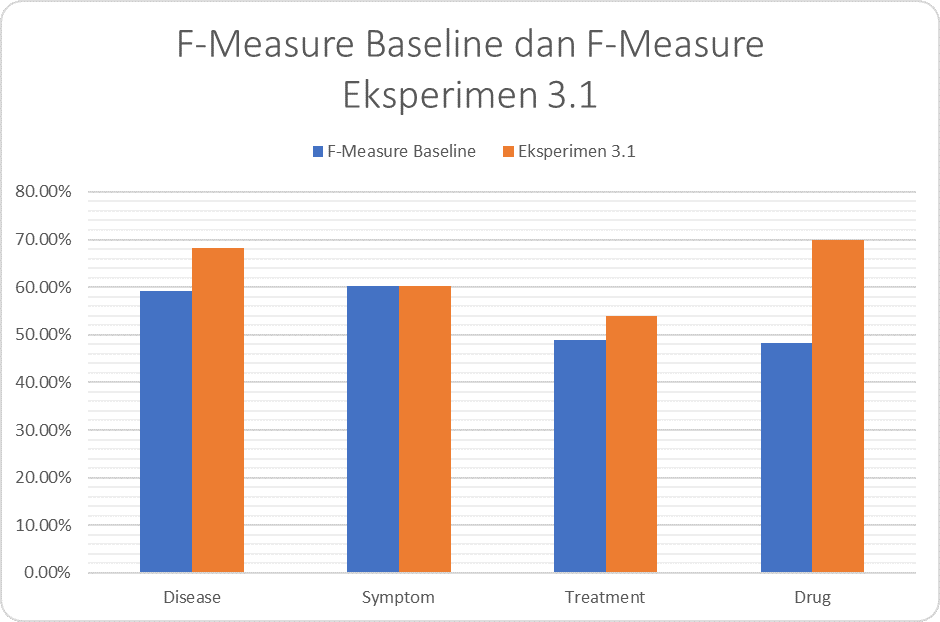
\includegraphics[width=0.85\linewidth]{images/histogram9}
%    	\caption{Histogram Perbandingan \textit{F-measure} \textit{Baseline} dengan Eksperimen 3.1}
%    	\label{fig:owndict9}
%    \end{figure}
%    
%    \subsubsection{Analisis}
%    Pada eksperimen ini, hasil yang sudah lebih baik apabila dibandingkan dengan hasil yang dicapai \cite{skripsiKakRadit} di entitas. Namun, dari eksperimen sebelumnya, terdapat akurasi yang turun, yaitu nilai \textit{precision} untuk entitas \textit{symptom}. Menurut \saya~hal ini terjadi karena informasi fitur yang berbeda-beda dijadikan satu, sehingga ada kemungkinan hilangnya informasi dari masing-masing fitur tersebut. Oleh karena itu, untuk mengatasi permasalahan tersebut \saya~mengusulkan arsitektur yang mana masing-masng kelompok fitur yang berbeda dipisahkan dan menjadi \textit{input} bagi masing-masing LSTMs. Untuk penjelasan eksperimen ini akan dijelaskan pada sub-eksperimen \ref{eks2:subeksrnn2}
%    
%    
%    \subsection{Eksperimen 3.2: Menguji Arsitektur LSTMs 2 Layer Multi-Input}\label{eks2:subeksrnn2}
%    %-----------------------------------------------------------------------------%
%    Pada sub-eksperimen sebelumnya, fitur-fitur yang berbeda digabung menjadi satu, sehingga ada kemungkinan hilangnya informasi dari fitur tersebut. Oleh karena itu, \saya~mengusulkan adanya layer tambahan setelah masing-masing fitur tersebut masuk ke dalam model. \Saya~mengusulkan bahwa masing-masing kelompok fitur menjadi \textit{input} LSTMs secara terpisah. Setelah masuk di RNNs, \textit{output} dari masing-masing LSTMs tersebut di-\textit{merge} ke dalam sebuah layer, lalu masuk kembali ke LSTMs untuk melihat konteks fitur-fitur sebelumnya. Dengan diusulkannya arsitektur RNNs ini \saya~berharap bahwa masing-masing fitur terjaga informasinya dan tidak terganggu dengan informasi lain.
%    
%    \subsubsection{Hasil Eksperimen}
%    \textbf{Waktu komputasi}: $ 20362.5 $ detik.
%    
%    Rangkuman hasil sub-eksperimen ini dapat dilihat pada Tabel \ref{table:owndict10} dan Gambar \ref{fig:owndict10}.
%        
%    \begin{table}
%    	\centering
%    	\caption{Tabel Hasil Eksperimen 3.2 dibandigkan dengan \textit{Baseline}}
%    	\begin{tabular}{|c|c|c|c|c|}
%    		\hline
%    		& \textit{Precision} & \f{\f{Recall}} & \f{\f{F-Measure}} \\ \hline
%    		\textit{Disease}      & 67.47\%             & 67.19\%        & 66.31\%           \\ \hline
%    		\textit{Symptom}      & 64.90\%             & 60.63\%        & 62.13\%           \\ \hline
%    		\textit{Treatment}    & 63.92\%             & 53.13\%        & 56.51\%           \\ \hline
%    		\textit{Drug}		  & 66.39\%             & 62.33\%        & 63.61\%           \\ \hline
%    		\textit{\textbf{Overall}}&\textbf{65.67\%}  & \textbf{60.82\%}& \textbf{62.14\%} \\ \hline
%    	\end{tabular}
%    	\label{table:owndict10}
%    \end{table}
%    
%    \begin{figure}
%    	\centering
%    	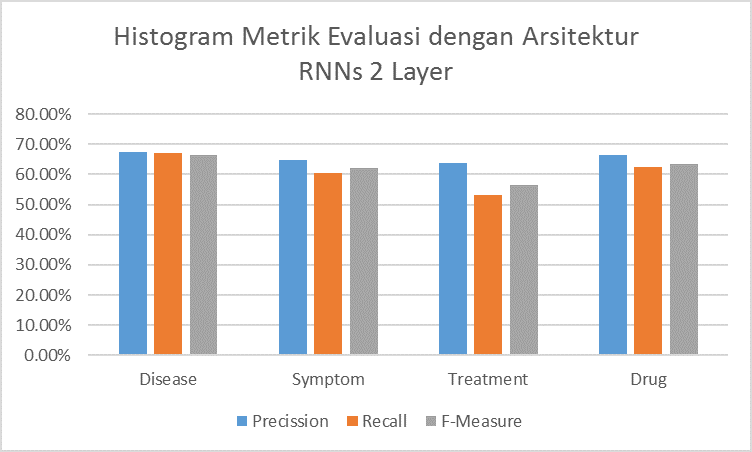
\includegraphics[width=0.85\linewidth]{images/histogramrnnv2}
%    	\caption{Histogram Perbandingan \textit{F-measure} \textit{Baseline} dengan Eksperimen 3.1, dan 3.2}
%    	\label{fig:owndict10}
%    \end{figure}
%
%	\subsubsection{Analisis}
%	Pada eksperimen ini, hasil yang sudah lebih baik apabila dibandingkan dengan hasil yang dicapai \cite{skripsiKakRadit} di masing-masing entitas dan lebih baik dibandingkan eksperimem \ref{eks2:subeksrnn1} pada identifikasi entitas \textit{symptom} dan \textit{treatment}.
